\documentclass[12pt]{article}
\usepackage{amssymb,amsmath,natbib,graphicx,amsthm,
  setspace,sectsty,anysize,times,dsfont,enumerate}

\usepackage[svgnames]{xcolor}

\usepackage{lscape,arydshln,relsize,rotating,multirow}
\usepackage{caption}
\captionsetup{%
  font=small,
  labelfont=normalfont,
  singlelinecheck=false,
  justification=justified
}
\usepackage{algorithm,algorithmic}

\graphicspath{{/Users/mtaddy/project/gamma_lasso/graphs/}}
\newtheorem{prop}{\sc Proposition}[section]
\newtheorem{theorem}{\sc Theorem}[section]
\newtheorem{definition}{\sc Definition}[section]
\newtheorem{lemma}{\sc Lemma}[section]
\newtheorem{corollary}{\sc Corollary}[section]

\marginsize{1.1in}{.9in}{.3in}{1.4in}

\newcommand{\nb}{\color{blue}}
\newcommand{\dbl}{\setstretch{1.5}}
\newcommand{\sgl}{\setstretch{1.2}}

\newcommand{\bs}[1]{\boldsymbol{#1}}
\newcommand{\mc}[1]{\mathcal{#1}}
\newcommand{\mr}[1]{\mathrm{#1}}
\newcommand{\bm}[1]{\mathbf{#1}}
\newcommand{\ds}[1]{\mathds{#1}}
\newcommand{\indep}{\perp\!\!\!\perp}
\DeclareMathOperator*{\argmin}{argmin}
\newcommand{\norm}[1]{|\!|#1|\!|_{1}}
\newcommand{\code}[1]{{\smaller\sf#1}}
\newcommand{\e}[1]{{\footnotesize$\times10$}{$^{#1}$}}

\usepackage[bottom,hang,flushmargin]{footmisc}

\pdfminorversion=4
\begin{document}
\setcounter{equation}{20}
\setcounter{section}{6}
\setcounter{table}{2}
\setcounter{figure}{3}
\sgl 

\pagestyle{empty}

~
\vskip .5cm

\noindent {\LARGE \bf Supplemental material} 

\vskip .25cm

\noindent{\LARGE \it One-step estimator paths for concave regularization

%\vskip .2cm \noindent Matt Taddy
}


\vskip 1cm


\setstretch{1.3}


\section{Implementation via coordinate descent}
\label{implement}

We use Coordinate descent \citep[CD; e.g.,][]{luenberger_linear_2008} to minimize
(3) at each step along the path. CD is a local optimization
algorithm that cycles through minimization of the conditional objective for
individual parameters when the remaining parameters are fixed. Algorithms of this type have have become popular in
$L_1$ penalized estimation since the work by \citet{friedman_pathwise_2007} and
\citet{wu_coordinate_2008}.

Our CD routine, outlined in Algorithm \ref{bmove}, is a solver for penalized
weighted-least squares problems as defined in equation (\ref{newton}) below.
This applies directly in Gaussian regression, and for non-Gaussian models  we
follow \citet{friedman_regularization_2010} and apply CD inside an outer loop
of iteratively re-weighted-least-squares \citep[IRLS;
e.g.,][]{green_iteratively_1984}. Given current parameter values
$\bs{\hat\beta}$, the Newton-Raphson update for maximum likelihood estimation
is $\bs{\beta} = \bs{\hat\beta} - \bm{H}^{-1}\bm{g}$, where $\bm{H}$ is the
information matrix with elements $h_{jk} = \partial^2 l/\partial
\beta_j\partial \beta_k |_{\bs{\hat\beta}}$ and $\bm{g}$ is coefficient
gradient (see Appendix \ref{models}). For exponential family linear models we
can write $\bm{H} = \bm{X}'\bm{V}\bm{X}$ and $\bm{g} = \bm{X}'\bm{V}(\bm{z} -
\bs{\hat\eta})$, where $\bm{V} = \mr{diag}(\bm{v})$, $\bm{v} = [v_1\ldots
v_n]$ are `weights', $\bm{z} = [z_1\ldots z_n]$ are transformed `response',
and $\hat\eta_i = \hat\alpha + \bm{x}_i\bs{\hat\beta}$.  In Gaussian
regression,  $v_i = 1$, $z_i=\hat\eta_i - y_i$, and the update is an exact
solution. For binomial regression, $v_i = q_i(1-q_i)$ and $z_i = \hat\eta_i -
(y_i-q_i)/v_i$, where $q_i = (1 + \exp[-\hat\eta_i])^{-1}$ is the  estimated
probability of success.

This yields $\bs{\beta} = (\bm{X}'\bm{V}\bm{X})^{-1}\bm{X}'\bm{V}\bm{z}$, such
that the Newton update solves a weighted-least-squares problem.   Adding $L_1$
costs,  the minimization objective from (3) becomes
\begin{equation} \label{newton}  \argmin_{\alpha,\beta_1 \ldots \beta_p \in
\ds{R}} \sum_i \frac{v_i}{2}(\alpha + \bm{x}_i'\bs{\beta} - z_i)^2  + n\sum_j \omega_j
\lambda |\beta_j|. \end{equation} Our solver iterates between CD on
(\ref{newton}) and,  for non-Gaussian models, updates to $\bm{v}$ and
$\bm{z}$. Each $t^{th}$ segment IRLS routine initializes $[\hat \alpha,
\bs{\hat \beta}]$ at solutions for $\lambda^{t-1}$, or at $[\hat \alpha,
\bm{0}]$ for $t=1$.  In the {\tt gamlr} implementation, a full pass update of
all parameters is done only at the first CD iteration; otherwise coordinates
with currently inactive (zero) $\hat\beta_j$ are not updated. Once the descent
converges for this {\it active set}, IRLS $\bm{v}$ and $\bm{z}$ are updated
and we begin a new CD loop with a full pass update.  The routine stops when
maximum squared change in $\beta_j$ scaled by its information over one of
these full pass updates is less than some tolerance threshold, ${\tt thresh}$.
The default in {\tt gamlr} uses a relative tolerance of $10^{-7}$ times null
model deviance.  

\vspace{.25cm}
\begin{algorithm}[ht]
\vspace{.25cm}
\caption{Coordinate descent\label{bmove}}

\vskip .15cm
\hskip .5cm Set ${\tt vh_j} = \sum_i v_i(x_{ij} - \bar x_j)^2$ 
and ${\tt vx_j} = \sum_i v_ix_{ij}$ for $j=1\ldots p$.

\vskip .15cm
\hskip .5cm while $\displaystyle \max_{j = 1\ldots p} {\tt vh_j}\Delta_j^2 > {\tt thresh}$:

\vskip .15cm
\hskip 1.5cm for {j=1\ldots p}:


\vskip .15cm
\hskip 2.5cm set ${\tt vg_j} = -\sum_i x_{ij}v_i(z_i-\hat\eta_i)$ and ${\tt ghb} = {\tt vg_j} - {\tt vh_j}\hat\beta_j$


\vskip .25cm
\hskip 2.5cm if $|{\tt ghb}| < n\lambda^t\omega^t_j$:~ $\Delta_j = -\hat\beta_j$

\vskip .1cm
\hskip 2.5cm else:~ $\Delta_j = -({\tt vg_j} - \mr{sign}({\tt ghb}) n\lambda^t\omega^t_j)/{\tt vh_j}$.

\vskip .25cm
\hskip 2.5cm  update $\hat\beta_j \stackrel{+}{=} \Delta_j$,
$\hat\alpha \stackrel{+}{=} -{\tt vx_j}\Delta_j$, 
and $\bs{\hat\eta} = \hat\alpha + \bm{X}'\bs{\hat\beta}$.

\vskip .25cm

\end{algorithm}


\subsection{Descent convergence}

 Despite the non-differentiability of $|\beta_j|$ at zero,
\citet{tseng_convergence_2001} establishes local convergence for CD on
(\ref{newton}) as a consequence of penalty separability: the
non-differentiable part of our objective is a sum of functions on only a
single coordinate.  Thus CD solves each weighted-least squares problem, and
the full algorithm converges if IRLS does.  For non-Gaussian models,
convergence of such nested $L_1$-penalized IRLS algorithms is shown
in \cite{lee_proximal_2014}.

\subsection{Quasi-Newton acceleration}
\label{qn}

Under high collinearity and large $\gamma$, one may wish to accelerate convergence via a quasi-Newton step
\citep[e.g.,][]{lange_numerical_2010}. Acceleration is applied to $\bs{\theta}
= [\alpha,\bs{\beta}]$, and a move is accepted only if it leads to a decrease
in the objective. Suppose that $\bs{\hat\theta}^{(0)}$,
$\bs{\hat\theta}^{(-1)}$, and $\bs{\hat\theta}^{(-2)}$ are the current,
previous, and previous-to-previous parameter estimates.  Write
$M(\bs{\hat\theta}^{(t)})$ as the implied CD update map $\bs{\hat\theta}^{(t)}
\rightarrow \bs{\hat\theta}^{(t+1)}$, such that the algorithm converges at
$\bs{\hat\theta} - M(\bs{\hat\theta}) = \bm{0}$.  With $\bm{u} =
\bs{\hat\theta}^{(-1)} - \bs{\hat\theta}^{(-2)}$ and $\bm{v} =
\bs{\hat\theta}^{(0)} - \bs{\hat\theta}^{(-1)}$, a secant approximation to the
gradient of $M$ is $\partial M/\partial \hat\theta_l \approx
\mr{v}_l/\mr{u}_l$.  An approximate Newton-Raphson step to solve for the root
of $\bs{\hat\theta} - M(\bs{\hat\theta}) $  updates each coordinate $\hat
\theta_l \gets \hat\theta_l^{(-1)} - (\hat\theta_l^{(-1)} -
\hat\theta_l^{(0)})/(1-\mr{v}_l/\mr{u}_l)$ which can be re-written as
$\hat\theta_l = (1-\mr{w}_l)\hat\theta_l^{(-1)} + \mr{w}_l\hat\theta_l^{(0)} $
where $\mr{w}_l = \mr{u}_l/(\mr{u}_l - \mr{v}_l)$.



\section{Gradient, curvature, and path starts}
\label{models}

The negative log likelihood objective in Gaussian regression is $
l(\alpha,\bs{\beta}) = 0.5\sum_i (y_i -\eta_i)^2 $ with gradient
$g_j(\bs{\beta}) = \partial l/\partial \beta_j = -\sum_i x_{ij}(y_i -
\eta_i)$, and coordinate curvature $h_j(\bs{\beta}) = \partial^2 l/\partial
\beta_j^2 = \sum_i x_{ij}^2$. In logistic regression, set $y_i = 1$ for
`success' and $y_i = 0$ for `failure' and write $q_i = (1 +
\exp[-\eta_i])^{-1}$ as the probability of success.  Then
$l(\alpha,\bs{\beta}) = \sum_i -y_i\eta_i + \log(1 +
  \exp[\eta_i])$,
$
g_j(\bs{\beta}) = \partial l/\partial \beta_j = -\sum_i
x_{ij}(y_i - q_i)$, and
$h_j(\bs{\beta}) = \partial^2 l/\partial \beta_j^2 = \sum_i
x_{ij}^2q_i(1-q_i)
$.
In each case, it is implied that $\hat\alpha$ has been set
to minimize $l(\alpha,\bs{\hat\beta})$. 

For $L_1$ costs $c_j(|\beta_j|) = |\beta_j|$, the infimum $\lambda$ such
that $\bs{\hat\beta} = \bm{0}$ is  available analytically as
$\lambda^1 =
n^{-1}\max\{|g_j(\bm{0})|,~j=1\ldots p\}$, the maximum mean
absolute gradient for the null model with $\bs{\beta} = \bm{0}$.  This formula
is used to obtain our starting values for the path algorithms.


\section{False Discovery Control}

A common goal in high-dimensional estimation is  support recovery -- having the set $\{j: \hat\beta_j \neq 0\} = \{j: \beta_j \neq 0\}$ for some `true' $\bs{\beta}$.
For standard lasso estimated $\bs{\hat\beta}$, many authors have shown \citep[e.g.,][]{buhlmann_statistics_2011,zou_adaptive_2006} that to get exact support recovery asymptotically or with high probability requires an {\it irrepresentability condition} which limits the size of least-squares projections from `true support' onto spurious covariates.  
\begin{definition} 
The $(\theta,S,\bm{v})$-irrepresentable condition for $\theta\in[0,1]$ and $\bm{v}\in \ds{R}^s$ holds that, 
\begin{equation}\label{irrep}
|\bs{x}_j'\bm{X}_S(\bm{X}_S'\bm{X}_S)^{-1}\bm{v}| \leq \theta ~~\forall~j\notin S
\end{equation}
\end{definition}
\noindent This is often presented with $\bm{v}=\bm{1}$.\footnote{\cite{wainwright_sharp_2009} shows that (\ref{irrep}) with $\theta=1$, $\bm{v}=\bm{1}$ is necessary for lasso sign recovery in the {\it noiseless} setting.} It
can be a strict design restriction; for example,
\citet{buhlmann_statistics_2011} show a single variable that is
highly correlated with many columns of $\bm{X}_S$ leading to failure. Much
of the literature on concave penalization has focused on achieving
support recovery {\it without} such conditions; see, e.g.,
\cite{fan_strong_2014} for a recent overview.  
Our results will require irrepresentable conditions with $\bm{v} =
\bs{\omega}_S$, which becomes less restrictive as one is able to shrink
weights $\omega_j$ for $j\in S$.  See the remarks for more discussion.

Our comparison of interest is between $\hat S = \{j:
\hat\beta_j \neq 0\}$, for $\bs{\hat\beta}$ from weighted-$L_1$ penalized
estimation, and $S = \{j:
\beta^\nu_j \neq 0\}$ for $\bs{\beta}^\nu$ the $L_0$ penalized estimator from
Theorem 3.1. Whether looking to an $L_0$ oracle or a sparse
truth, our experience is that exact support recovery does not occur in
practice   (e.g., see the simulation in Section 5).  Thus, we instead 
focus on ability of the weighted-lasso to minimize {\it false discoveries}:
$\hat\beta_j
\neq 0$ when $\beta^\nu_j=0$. 

\begin{theorem}
Consider the setting of Theorem 3.1. 
If $\omega_{S^c}^{\mr{min}} = 1$ and $\lambda > \sqrt{2\nu}$ then
\begin{equation}\label{falsepos}
\|\bm{X}_{S^c}'\bm{X}_S(\bm{X}_S'\bm{X}_S)^{-1}\bs{\omega}_S\|_{\infty} \leq 1 - \frac{\sqrt{2\nu}}{\lambda_t} ~~\Rightarrow~~\hat S \cap S^c = \varnothing.
\end{equation}
\end{theorem}
\noindent The result follows directly from the sign recovery lemma \ref{signrecov}. 

\vskip .25cm
\noindent {\bf Remarks}
\vskip .25cm
\noindent $\bullet$~~ 
From Theorem 7.4 in \cite{buhlmann_statistics_2011}, 
the irrepresentability condition holds with 
$|\bs{x}_j'\bm{X}_S(\bm{X}_S'\bm{X}_S)^{-1}\bs{\omega}_S|
\leq \frac{\|\bs{\omega}_S\|}{\sqrt{s}}\theta_{\mr{adap}}(S)$ where $\theta_{\mr{adap}}(S)$ is their `adaptive restricted regression' coefficient.  Of interest here, they show that $\theta_{\mr{adap}}(S) \leq \sqrt{s}/\Lambda_{\mr{min}}(S)$ where $\Lambda_{\mr{min}}(S)$ is the minimum eigenvalue of $\bm{X}_S'\bm{X}_S/n$.  Thus, $(i)$ can be replaced by the restriction $\Lambda_{\mr{min}}(S) \geq \|\bs{\omega}_S\|(1 - \sqrt{2\nu}/(\omega_{S^c}^{\mr{min}}\lambda))^{-1} = \sqrt{s}L$, with $L$ from Theorem 3.1, and small values for $L$ appear key in both predictive performance and support recovery.

\vskip .25cm
\noindent $\bullet$~~ Without irrepresentability,  limits on false discovery are more pessimistic.  Convergence
conditions imply that for $j \in S^c \cap \hat S$ we have
$n\lambda \omega_j = |\bs{x}_j'(\bm{X}\bs{\hat\beta}-\bm{y})| \leq
|\bs{x}_j'\bm{X}(\bs{\hat\beta}-\bs{\beta}^\nu)| + |\bs{x}_j'\bm{e}^S| \leq
n\left(2\|\bs{\omega}_S\|/\phi(L,S) + \sqrt{2\nu}/\lambda\right) ~\forall~j$. 
Dividing by $n\lambda\omega_j$ and counting yields
\begin{equation}\label{pessimism}
|S^c \cap \hat S| \leq \left|\frac{1}{\bs{\omega}_{S^c \cap \hat S}}\right|
\left(\frac{2\|\omega_S\|}{\phi(L,S)} + \frac{\sqrt{2\nu}}{\lambda}\right)
\end{equation}
Without the ability to
make $\omega_j$ very big for $j \in S^c$ (e.g., as in a thresholding procedure
like that of \citealt{zhou_thresholding_2009}), the result in (\ref{pessimism}) has little to say about false discovery control.

\subsection{Sign Recovery}

\begin{lemma}\label{signrecov}
Under the setting of Theorem 3.1, with $\hat S = \{j:\hat\beta_j \neq 0\}$, if $\omega_{S^c}^{\mr{min}}\lambda > \sqrt{2\nu}$ then
\begin{equation}
|\bs{x}_j'\bm{X}_S(\bm{X}_S'\bm{X}_S)^{-1}\bs{\omega}_S| \leq 1 - \frac{\sqrt{2\nu}}{\lambda\omega_j}~~\forall~j ~\in~S^c \Rightarrow \hat{S} \cap S^c = \varnothing.
\end{equation}
 If in addition
$\left|(\bm{X}_S'\bm{X}_S)^{-1}\bm{X}_S'\bm{y}\right|_\infty > n\lambda\left|(\bm{X}_S'\bm{X}_S)^{-1}\bs{\omega}_S\right|_\infty$, then 
$\mr{sgn}(\bs{\hat\beta}) = \mr{sgn}(\bs{\beta}^\nu)$.
\end{lemma}
\begin{proof} 
The Karush-Kuhn-Tucker (KKT) conditions at weighted-$L_1$ minimization convergence imply that 
\begin{equation}
\bm{x}_j'\bm{X}(\bs{\hat\beta}-\bs{\beta}^\nu) + \bm{x}_j'\bm{e}^S = -n\lambda\zeta_j~~\text{for}~~j=1\dots p
\end{equation} where $|\zeta_j| = \omega_j$ for $j\in\hat S$ and $|\zeta_j| \leq \omega_j$ for $j\in\hat S^c$.  Following  closely related proofs in \cite{wainwright_sharp_2006,wainwright_sharp_2009,zhou_adaptive_2009}, 
$\hat{S} \cap S^c = \varnothing$ occurs if and only if these KKT conditions
hold for projections restricted to $S$,
\begin{equation}
\bm{X}_S'\bm{X}_S(\bs{\hat\beta}_S-\bs{\beta}^\nu_S) + \bm{X}_S'\bm{e}^S =-n\lambda\bs{\zeta}_S ~~\Rightarrow~~ \bs{\hat\beta}_S-\bs{\beta}^\nu_S = -n\lambda(\bm{X}_S'\bm{X}_S)^{-1}\bs{\zeta}_S.
\end{equation}
Thus all of the spurious regressors in $S^c$ will have $\hat \beta_j = 0$
if and only if
\begin{equation}
\bs{x}_j'\bm{X}_S(\bs{\hat\beta}_S-\bs{\beta}^\nu_S) - \bs{x}_j'\bm{e}^S 
\leq n\lambda\zeta_j ~~\Leftarrow~~
1 - \frac{|x_j'\bm{e}^S|}{n} \geq 1 - \frac{\sqrt{2\nu}}{\lambda\omega_j} \geq |\bs{x}_j'\bm{X}_S(\bm{X}_S'\bm{X}_S)^{-1}\bs{\omega}_S|.
\end{equation}
Finally, for sign recovery on $j\in S$ we need 
$
|\beta_j^\nu| - |\beta^\nu_j - \hat\beta_j| > 0 ~~\forall~j~\in~S
$,
and our stated condition follows from  $\bs{\beta^\nu}_S =
(\bm{X}_S'\bm{X}_S)^{-1}\bm{X}_S'\bm{y}$ and $ \bs{\beta^\nu}_S-
\bs{\hat\beta}_S = n\lambda (\bm{X}_S'\bm{X}_S)^{-1}\bs{\zeta}_S$.
\end{proof}

\section{Extra proofs}

\subsection{Stagewise Regression}

Theorem 3.1 uses the following simple result for stagewise regression -- iterative fitting of new covariates to the residuals of an existing linear model (as in, e.g., \citealt{goldberger_stepwise_1961}). 
\begin{lemma}\label{SSElemma}
Say $\mr{MSE}_S = \|\bm{X}\bs{\beta}^S-\bm{y}\|^2/n$ and 
$\mr{cov}(\bs{x}_j,\bm{e}^S) = \bs{x}_j'(\bm{y}-\bm{X}\bs{\beta}^S)/n$ are sample variance and covariances.  Then for any $j \in 1\ldots p$, 
\[
\mr{cov}^2(\bs{x}_j,\bm{e}^S) \leq \mr{MSE}_S - \mr{MSE}_{S\cup j}
\]
\end{lemma}
\begin{proof}
From the well-known property on the correlation coefficient ($R^2$) for linear models,   
in-sample correlation and variances are such that
\[
\frac{\mr{cov}^2(\bs{x}_j,\bm{e}^S)}{\mr{var}(\bs{x}_j)\mr{var}(\bm{e}^S)} = 1 - \frac{\mr{var}(\bm{e}^S-\tilde\beta_j\bs{x}_j)}{\mr{var}(\bm{e}^S)}
\]
where $\tilde\beta_j = \bs{x}_j'\bm{e}^S/(\bs{x}_j'\bs{x}_j)$ is the stagewise coefficient estimate.  Since $\mr{var}(\bs{x}_j)=1$, multiplying everything by $\mr{var}(\bm{e}^S)$ yields $\mr{cov}^2(\bs{x}_j,\bm{e}^S) =
\mr{var}(\bm{e}^S) - \mr{var}(\bm{e}^S-\tilde\beta_j\bs{x}_j)
\leq \mr{var}(\bm{e}^S) - \mr{var}(\bm{e}^{S\cup j})$.
The last inequality holds because $\bm{e}^{S\cup j}$, residuals from OLS on $\bm{X}_{S\cup j}$, have the smallest-possible sum of squares for that set of covariates.  With $\mr{var}(\bm{e}^S) = \mr{MSE}_S$, etc, we are done.
\end{proof}

\subsection{Bayesian MAP}

\begin{prop}\label{penprop}
  $\bs{\hat\beta}$ solves (14) if and only if it is also in the
  solution to (13).
\end{prop}
\begin{proof}
  The conditional posterior mode for each $\tau_j$ given $\beta_j$
  is $\tau(\beta_j) = \gamma s/(1 + \gamma|\beta_j|)$.  Any joint solution
  $[\bs{\hat\beta},\bs{\hat\tau}]$ for (13) thus
  consists of $\hat{\tau}_{j} = \tau(\hat\beta_{j})$;
  otherwise, it is always possible to decrease the objective by
  replacing $\hat\tau_{j}$. Setting each $\tau_j = 
  \tau(\beta_j)$ in (13) and removing constant terms yields
  (14).  Moreover, the solution to (13) solves
  (14): otherwise, there would need to be a point on the profile
  slice of (13) defined by $\tau_{j} =
  \tau(\hat\beta_{j})$ that is lower than its minimum.
\end{proof}

For a Bayesian it is odd to be solving for $\bs{\tau}$ rather than
marginalizing over its uncertainty.  However, recognizing the form of a gamma
density  in (12), $\pi(\beta_j,\tau_j)$ integrates over $\tau_j$ to
yield the marginal prior $ \pi(\beta_j) = 0.5s\left( 1+
\gamma|\beta_j|\right)^{-(s+1)}$. This is the generalized double Pareto
density, as in  \citet{armagan_generalized_2013}. Since $-\log \pi(\beta_j)
\propto (s+1)\log(1 + \gamma|\beta_j|)$, the {\it profile} MAP solution to
(13) is also the {\it marginal} MAP for
$\bs{\beta}$ under $\mr{Ga}(s-1,1/\gamma)$ priors on each $\tau_j$.




\section{Stability}

A strong form of stability comes from convexity of the penalized objective in
(1). This requires that the minimum eigenvalue of
$\bm{H}(\bs{\beta})$, the Hessian matrix of second derivatives of
$l(\bs{\beta})$, is greater than $|c''(\beta_j)| ~\forall j$.  For penalized
least-squares under log costs, this amounts to requiring that the minimum
eigenvalue of $\bm{H} = \bm{X}'\bm{X}$ is greater than
$\lambda\gamma^2$.\footnote{ If $\nu$ is an eigenvalue of $\bm{H}$, then
$(\bm{H} -
\nu \bm{I})\bm{v} = 0$ for some nonzero $\bm{v}$; the negative log posterior
Hessian at zero is $\bm{H} - \lambda\gamma^2\bm{I}$ and $(\bm{H} -
\lambda\gamma^2\bm{I} + s\gamma^2\bm{I} -
\nu \bm{I})\bm{v} = 0$ so that 
$\nu - s\gamma^2$ is an eigenvalue of the minimization objective.  }  In the
simple {\it standardized orthogonal covariate} case, this has an easy
interpretation in the context of our Bayesian model from Section 4.1:
for Gaussian regression, $h_j = \sum_i x_{ij}^2 = n$ and the objective is
convex if prior variance on each $\tau_j$  is less than the number of
observations.  For logistic regression you need $\mr{var}(\tau_j) < n/4$,
since $\bm{H}$ now depends upon the coefficient values.

In real examples, however, we cannot rely upon objective convexity. A more
useful definition of stability requires continuity of the implied  coefficient
function, $\hat\beta(\bm{y})$, in an imagined univariate regression problem
(or for orthogonal covariates).  This is one of the key requirements of
concave penalties listed by \citet{fan_variable_2001}. Many popular concave
cost functions, such as the SCAD and MCP, have been engineered to have this
continuity property. Conveniently, \cite{zou_one-step_2008} show that OSE LLA
solutions have this property even if the target objective does not.  For
example, even though the log penalty {\it does not} generally lead to
continuous thresholding, their result implies that the GL solutions are
continuous for $\gamma<\infty$.

A theoretically richer form of stability is Lipschitz continuity of the
implied prediction function, $\boldsymbol{\hat y} = \bm{X}\boldsymbol{\hat
\beta}(\bm{y})$, which requires that   $
\|\bm{\hat y}(\bm{y}_1)-\bm{\hat y}(\bm{y}_2)| \leq L\|\bm{y}_1-\bm{y}_2\| $
for some finite constant $L$ on all possible $\bm{y}_1,\bm{y}_2$.
\citet{zou_degrees_2007} establish Lipschitz continuity for $L_1$ estimated
predictors as part of their derivation of a degrees-of-freedom estimator.
Thus, conditional upon values for the coefficient-specific weights, POSE and
GL are trivially Lipschitz continuous.  Unconditionally, we do not believe
that the paths have this guarantee.  However, we'll see in the next section
that a heuristic degrees-of-freedom estimator that takes such stability for
granted performs well as the basis for model selection.

Finally, the basic and most important type of stability is practical path continuity: by this, we mean that solutions change slowly enough along the path so that computational costs are kept within budget.   A regularization path can be built from a continuous thresholding function, or perhaps even be Lipschitz stable, but 
none of that matters if it takes too long to fit.  For example, Figure \ref{nhltime} shows timings growing rapidly with large $\gamma$ for the hockey data  of Section 6, even though all of these specifications are theoretically stable by some criteria.

\begin{figure}[bht]
\vskip -.5cm
\centering
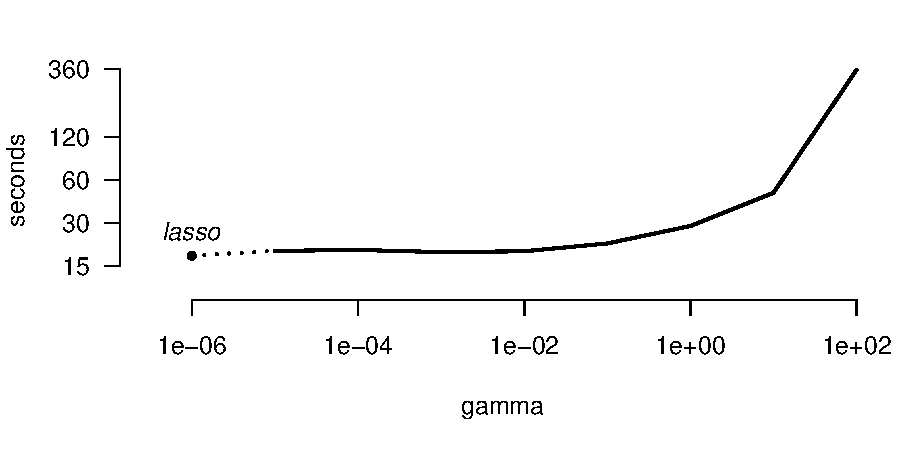
\includegraphics[width=5in]{graphs/nhl_time}
\vskip -.25cm
\caption{\label{nhltime} 
Timings for the hockey data path fits of Section 6
on a length-100 grid with $\lambda^{100} = 0.01\lambda^1$. }
\vskip -.25cm
\end{figure}



\section{Information Criteria}


We would like to choose a model that performs well in predicting new data.
 `Good prediction' can be measured in a variety of ways.  A common and
 coherent framework is to consider minimizing Kullback-Leibler (KL)
 divergence.  Say $g(\bm{y})$ is the true data generating process, and
 $f(\bm{y}; \bs{\eta},\phi)$ is the parametric density under study, which we
 suppose here is a natural exponential family  with $\ds{E}[\bm{y}]=\bs{\eta}$
 and dispersion $\phi$. Then we wish to minimize
\begin{equation}
\mr{KL}(\bs{\eta},\phi) = \ds{E}_g \log g(\bm{y}) - \ds{E}_g \log f(\bm{y}; \bs{\eta},\phi),
\end{equation}
the expected difference between log true density and our parametric approximation.  Since $\ds{E}_g \log g(\bm{y})$ is constant, this leads one to minimize 
$Q(\bs{\eta},\phi) = -\ds{E}_g \log f(\bm{y}; \bs{\eta},\phi)$, the expected negative log likelihood.   There is no requirement that $g$ is a member of the family defined by $f$.

If parameters are to be estimated as $[\bs{\eta}_{\bm{y}},\phi_{\bm{y}}]$, functions of random sample $\bm{y} \sim g$, then $Q(\bs{\eta}_{\bm{y}},\phi_{\bm{y}})$ is itself a random variable and one chooses estimators to minimize its expectation.  {\it Crucially, we imagine a double-sample expectation}, where the minimization objective is
\begin{equation}\label{dualexpect}
\ds{E}_{\bm{y}|g} \ds{E}_{\bm{\tilde y}|g} \log f(\bm{\tilde y}; \bs{\eta}_{\bm{y}},\phi_{\bm{y}}).
\end{equation}
The notation here indicates that inner and outer expectations are based on two {\it independent} random samples from $g$: $\bm{y}$ for training, upon which $\bs{\eta}_{\bm{y}},\phi_{\bm{y}}$ are calculated, and $\bm{\tilde y}$ for validation.  

Information criteria (IC) are analytic approximations to metrics like
(\ref{dualexpect}).\footnote{Not all IC target (\ref{dualexpect}).  For
example, the `Bayesian' BIC, with  $c(df) =\log(n)df$
\citep{schwarz_estimating_1978}, is derived
\citep{kass_bayes_1995} as Laplace approximation to the negative log of the
 {\it marginal likelihood}.  We include the BIC as a comparator to AIC and
 AICc in our examples. }  They take the form
\begin{equation}\label{ic}
 -2\log f(\bm{y}; \bs{\eta}_{\bm{y}},\phi_{\bm{y}}) + c(df)
 \end{equation} 
where $c(df)$ is cost of the {\it degrees-of-freedom} used in
$\bs{\eta}_{\bm{y}}$ -- e.g., for $\bm{y} \sim (\bs{\eta},\sigma^2\bm{I})$,
\citet{efron_least_2004} defines $df =
\sigma^{-2} \sum_i \mr{cov}(\eta_{\bm{y}i}, y_i)$. 

Consider a Gaussian regression model where $\bs{\eta}_\bm{y}$ is an estimate
for $\bs{\eta} = \ds{E}\bm{y}$ using $df$ degrees of freedom, and set $\phi_\bm{y} =
\sigma^2_{\bm{y}} = \sum_i (y_i - \eta_{\bm{y}i})^2/n$. We'll derive
\begin{equation}\label{aiccapprox}
df\frac{n}{n-df-1}  \approx \ds{E}_{\bm{y}|g}\left[\log f(\bm{y}; \bs{\eta}_{\bm{y}},\phi_{\bm{y}}) - \ds{E}_{\bm{\tilde y}|g} \log f(\bm{\tilde y}; \bs{\eta}_{\bm{y}},\phi_{\bm{y}})
\right],
\end{equation}
such that AICc's complexity penalty is the expected bias that results from taking the fitted log likelihood as an estimate for (\ref{dualexpect}).  First, by cancellation the inner term of (\ref{aiccapprox}) simplifies as 
\begin{equation}
\log f(\bm{y}; \bs{\eta}_{\bm{y}},\phi_{\bm{y}}) - \ds{E}_{\bm{\tilde y}|g} \log f(\bm{\tilde y}; \bs{\eta}_{\bm{y}},\phi_{\bm{y}}) = 
\frac{\ds{E}_{\bm{\tilde y}|g} \sum_i (\tilde y_i - \eta_{\bm{y}i})^2}{2 \sigma^2_{\bm{y}}} - \frac{n}{2}.
\end{equation}
Now, assume that the {\it true} model is linear and that the data were generated
from $\bm{y}\sim g(\bs{\eta}, \sigma^2\bm{I})$.  The \cite{mallows_comments_1973} $C_p$ formula holds that 
$n\sigma^2_{\bm{y}} + 2 \sigma^2 df$ is an unbiased estimator for  expected 
sum of square errors $\ds{E}_{\bm{\tilde y}|g} \sum_i (\tilde y_i - \eta_{\bm{y}i})^2/n$, such that
\begin{equation}
\frac{\ds{E}_{\bm{\tilde y}|g} \sum_i (\tilde y_i - \eta_{\bm{y}i})^2}{2 \sigma^2_{\bm{y}}} - \frac{n}{2} 
 ~\approx~ \frac{n\sigma^2_{\bm{y}} + 2 \sigma^2 df}{2 \sigma^2_{\bm{y}}} - \frac{n}{2}
 ~=~  df\frac{\sigma^2 }{\sigma^2_{\bm{y}}}.
\end{equation}
At this point, we see that the standard AIC approximation results from equating $\sigma^2 \approx \ds{E}_{\bm{y}|g}\sigma^2_{\bm{y}}$, so that $df\ds{E}_{\bm{y}|g}[\sigma^2/\sigma^2_{\bm{y}}] \approx df$.  This will underpenalize complexity whenever residual variance $\sigma^2_{\bm{y}}$ tends to be smaller than the true variance $\sigma^2$  -- that is, whenever the model is overfit.  In contrast, AICc applies the chi-squared goodness of fit result $
{n\sigma^2_{\bm{y}}/\sigma^2} \sim \chi^2_{n-df-1}
$
to obtain 
\begin{equation}
\ds{E}_{\bm{y}|g}\left[\frac{\sigma^2 }{\sigma^2_{\bm{y}}}df\right]= 
n\ds{E}_{\bm{y}|g}\left[\frac{1}{n\sigma^2_{\bm{y}}/\sigma^2}\right]df = 
\frac{n}{n-df-1}df.
\end{equation}
Multiplying by $-2$ and subtracting from $-2\log f(\bm{y}; \bs{\eta}_{\bm{y}},\sigma_{\bm{y}})$ yields the AICc.


\section{Hockey players}

Ten-fold CV results are shown in Figure
\ref{nhlcv} for $\gamma$ of 0, 1, and 10.  The OOS error minima are around the
same in each case -- average deviance slightly above 1.16 -- but errors
increase much faster away from optimality with larger $\gamma$.   We also see
that AICc selection is always between the CV.min and CV.1se selctions:  at
$\gamma=0$ AICc matches the CV.1se choice, while at $\gamma=10$ it has moved
right to the CV.1se  selection.  Our heuristic might be
over-estimating $df$ for large-$\gamma$ models (especially under this very
collinear design), but one would also suspect that CV estimates of minimum
deviance are biased downward more dramatically for larger $\gamma$ than for
low-variance small-$\gamma$ estimators.


\begin{figure}[h!]
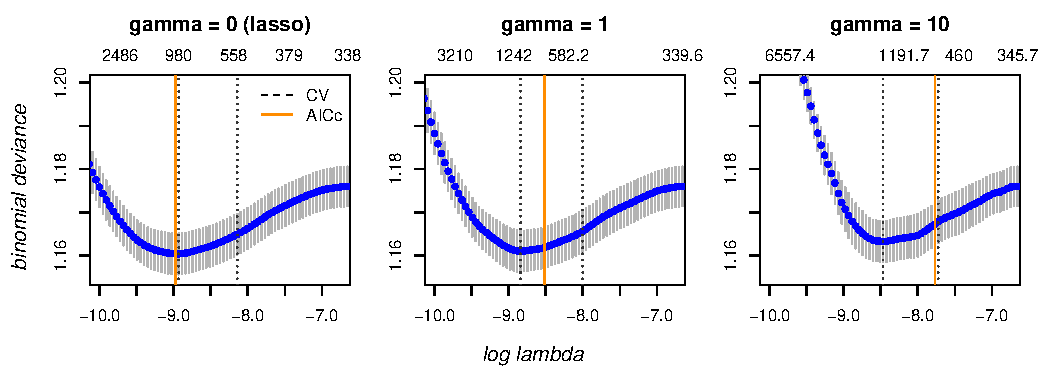
\includegraphics[width=\textwidth]{graphs/nhl_cv}
\caption{\label{nhlcv} Hockey example 10-fold CV: mean OOS deviance $\pm 1$se, with minimum-error and 1SE selection rules marked with black dotted lines, and solid orange line showing AICc selection. }
\end{figure}


\section{Full simulation results}

Continuous-response data are simulated from
 a $p=1000$ dimensional linear model
\begin{align}
\label{simdgp-both}
y &\sim \mr{N}\left(\bm{x}'\bs{\beta},\sigma^2\right) ~~\text{where}~~
\beta_j = \frac{1}{j}\exp\left(-\frac{j}{{\sf d}} \right)\text{for}~~j=1\dots p~~\text{and,~given~}\bm{z} \sim \mr{N}\left(\bm{0},\bs{\Sigma}\right)\notag,\\
&\text{either}~~\textit{dense design:~~} x_j=z_j ~~\text{or}~~ \textit{sparse design:~~} 
x_j \stackrel{ind}{\sim} \mr{Bern}\left( 1/(1+e^{-z_j})\right).
\end{align}

\vspace{-.4cm}
\noindent
Each simulation draws $n=1000$ means $\eta_i =
\bm{x}_i'\bs{\beta}$, and two independent response samples 
$\bm{y},\bm{\tilde y} \sim \mr{N}(\bs{\eta},\sigma^2\bm{I})$. Residual
variance $\sigma^2$ and covariate correlation $\bs{\Sigma}$ are adjusted across
runs.  In the first case, we define $\sigma^2$ through {\it signal-to-noise}
ratios $\mr{sd}(\bs{\eta})/\sigma$ of $1/2$, $1$, and $2$.  In the latter
case, multicollinearity is parametrized via $\Sigma_{jk} =
\rho^{|j-k|}$, and we consider $\rho = 0, 0.5,~\text{and}~0.9$.
Finally, the coefficient decay rate ${\sf d}$ controls the effective sparsity: how much $\bs{\beta}$ is \textit{measurably} different from zero. See Figure \ref{fig:betadecay} for illustration; we consider
${\sf d}$ of $10$, $50$, $100$, and $200$.

\begin{figure}[h]\centering
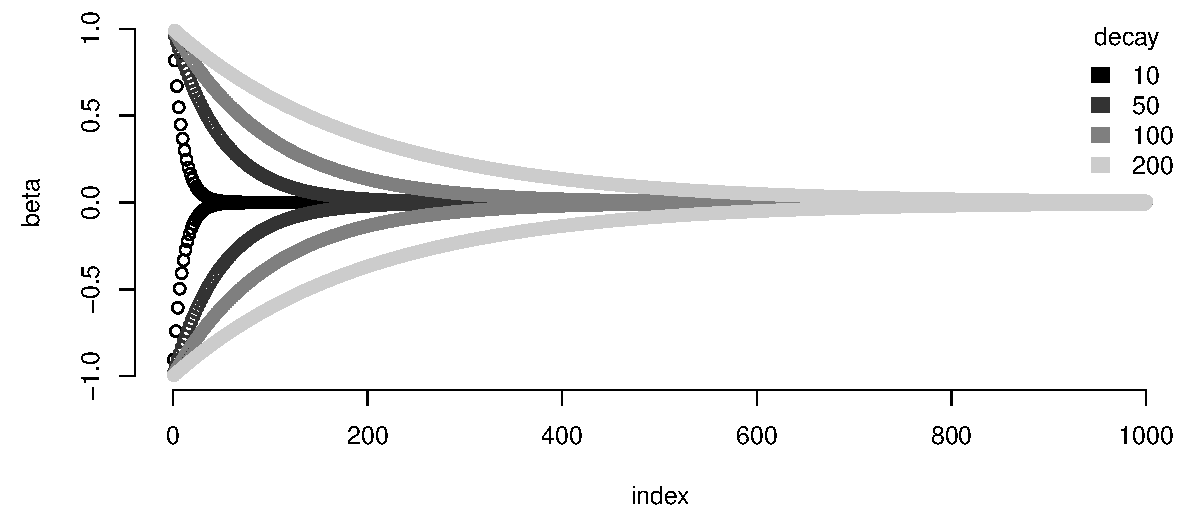
\includegraphics[width=.8\textwidth]{graphs/betadecay}
\caption{\label{fig:betadecay} The linear model coefficients for our simulation in \ref{simdgp-both}.}
\end{figure}
% pdf("betadecay.pdf",width=8,height=3.5)
% par(mai=c(.9,.9,.1,.1))
% j <- 1:1000
% b <- function(d){ ((-1)^j)*exp(-j/d) }
% plot(j, b(10), bty="n",xlab="index",ylab="beta", ylim=c(-1,1))
% points(j, b(50), col="grey20")
% points(j, b(100), col="grey50")
% points(j, b(200), col="grey80")
% legend("topright", bty="n", fill=paste("grey",c(0,20,50,80),sep=""),legend=c(10,50,100,200),title="decay",border=0)
% dev.off()

Results for both sparse and dense designs, over a set of 1000 datasets, are presented in the following tables.  We first report out-of-sample $R^2 = 1 -
\mr{var}(\bm{\tilde y} - \bs{\eta}_\bm{y})/\mr{var}(\bm{\tilde y})$, followed by tables showing false discovery and sensitivity with respect to the $C_p$
oracle. 


\setstretch{1}
\bibliographystyle{chicago}
\bibliography{pose}


% dense version of paper table
\begin{table}
\vspace{-.2cm}
\footnotesize
\begin{center}
\begin{tabular}{ccc|cc|cc|cc|cc|c|c}
\hline &&&\multicolumn{9}{|c|}{~}\\[-1ex]
\multicolumn{3}{c}{~}&\multicolumn{9}{|c|}{\bf \% Worse than oracle $\boldsymbol{C_p}$  } &   \\[1ex]
& &
& \multicolumn{2}{c}{lasso} 
& \multicolumn{2}{c}{GL $\gamma=1$} 
& \multicolumn{2}{c}{GL $\gamma=10$} 
& \multicolumn{2}{c}{marginal AL} 
& \multicolumn{1}{c|}{~} & \\[-0.5ex]
$\mr{sd}(\bs{\eta})/\sigma$ & {\sf d} & $\rho$ 
& ~~~\scriptsize\it AICc & \multicolumn{1}{c}{\scriptsize\it CV~~~}
& ~~~\scriptsize\it AICc & \multicolumn{1}{c}{\scriptsize\it CV~~~}
& ~~~\scriptsize\it AICc & \multicolumn{1}{c}{\scriptsize\it CV~~~}
& ~~~\scriptsize\it AICc & \multicolumn{1}{c}{\scriptsize\it CV~~~} 
& \multicolumn{1}{c|}{ MCP} & $C_p$ $R^2$ \\[.5ex]
\hline\rule{0pt}{3ex}
& & \it  0  & 3 & 3 & 2 & 2 & 2 & {\bf 1} & 2 & 2 & {\bf 1} & \it  0.79 \\
 & \it  10  & \it  0.5  & 5 & 5 & 4 & 4 & 3 & {\bf 2} & 8 & 8 & {\bf 2} & \it  0.79 \\
& & \it  0.9  & 7 & 6 & 6 & 5 & 4 & 4 & 10 & 10 & {\bf 3} & \it  0.79 \\[1ex]
\cline{2-3}\rule{0pt}{3ex}
& & \it  0  & 6 & 5 & 5 & {\bf 4} & 5 & 5 & 5 & 5 & {\bf 4} & \it  0.77 \\
\it  2  & \it  50  & \it  0.5  & 11 & 8 & 9 & 7 & {\bf 6} & {\bf 6} & 14 & 14 & {\bf 6} & \it  0.77 \\
& & \it  0.9  & 14 & 10 & 11 & 9 & {\bf 7} & {\bf 7} & 44 & 44 & {\bf 7} & \it  0.77 \\[1ex]
\cline{2-3}\rule{0pt}{3ex}
& & \it  0  & 9 & 6 & 7 & {\bf 5} & 7 & 7 & 8 & 7 & {\bf 5} & \it  0.75 \\
 & \it  100  & \it  0.5  & 18 & {\bf 9} & 13 & {\bf 9} & {\bf 9} & {\bf 9} & 21 & 17 & {\bf 9} & \it  0.75 \\
& & \it  0.9  & 23 & 11 & 16 & 10 & 10 & {\bf 9} & 56 & 56 & 11 & \it  0.75 \\[1ex]
\cline{2-3}\rule{0pt}{3ex}
& & \it  0  & 11 & {\bf -1} & 6 & 0 & 3 & 7 & 6 & 2 & {\bf -1} & \it  0.67 \\
 & \it  200  & \it  0.5  & 47 & {\bf 5} & 20 & 7 & 6 & 74 & 30 & 21 & {\bf 5} & \it  0.67 \\
& & \it  0.9  & 90 & 39 & 84 & 42 & {\bf 7} & 92 & 66 & 67 & 58 & \it  0.68 \\[1ex]
\cline{2-3}\hline\rule{0pt}{3ex}
& & \it  0  & 9 & 9 & 7 & 7 & 8 & 6 & 9 & 10 & {\bf 5} & \it  0.48 \\
 & \it  10  & \it  0.5  & 16 & 16 & 14 & 13 & 10 & 9 & 18 & 18 & {\bf 7} & \it  0.48 \\
& & \it  0.9  & 23 & 22 & 20 & 19 & 16 & 14 & {\bf 10} & {\bf 10} & 11 & \it  0.48 \\[1ex]
\cline{2-3}\rule{0pt}{3ex}
& & \it  0  & 19 & {\bf 17} & 18 & {\bf 17} & 27 & 23 & {\bf 17} & 18 & {\bf 17} & \it  0.44 \\
\it  1  & \it  50  & \it  0.5  & 38 & 32 & 32 & 29 & 28 & 34 & 39 & 38 & {\bf 25} & \it  0.44 \\
& & \it  0.9  & 70 & 68 & 70 & 54 & 66 & 56 & 46 & 46 & {\bf 31} & \it  0.44 \\[1ex]
\cline{2-3}\rule{0pt}{3ex}
& & \it  0  & 26 & {\bf 20} & 24 & 25 & 45 & 52 & 22 & 22 & {\bf 20} & \it  0.40 \\
 & \it  100  & \it  0.5  & 64 & 57 & 56 & 61 & 51 & 95 & 51 & {\bf 47} & 57 & \it  0.40 \\
& & \it  0.9  & 86 & 88 & 90 & 88 & 89 & 88 & {\bf 65} & 67 & 85 & \it  0.40 \\[1ex]
\cline{2-3}\rule{0pt}{3ex}
& & \it  0  & 35 & {\bf 21} & 27 & 47 & 66 & 94 & 23 & {\bf 21} & {\bf 21} & \it  0.34 \\
 & \it  200  & \it  0.5  & 84 & 87 & 93 & 94 & 84 & 99 & 58 & {\bf 52} & 87 & \it  0.34 \\
& & \it  0.9  & 91 & 93 & 95 & 93 & 96 & 94 & {\bf 81} & 83 & 93 & \it  0.34 \\[1ex]
\cline{2-3}\hline\rule{0pt}{3ex}
& & \it  0  & 27 & 28 & 27 & {\bf 24} & 48 & 25 & 44 & 56 & {\bf 24} & \it  0.17 \\
 & \it  10  & \it  0.5  & 50 & 52 & 46 & 45 & 63 & 41 & 71 & 77 & {\bf 29} & \it  0.17 \\
& & \it  0.9  & 44 & 45 & 44 & 43 & 42 & 42 & 29 & {\bf 28} & 38 & \it  0.18 \\[1ex]
\cline{2-3}\rule{0pt}{3ex}
& & \it  0  & {\bf 55} & 57 & 74 & 71 & 101 & 94 & 72 & 90 & 58 & \it  0.13 \\
\it  0.5  & \it  50  & \it  0.5  & {\bf 90} & 95 & 98 & 96 & 101 & 100 & 108 & 117 & 95 & \it  0.13 \\
& & \it  0.9  & 79 & 80 & 81 & 79 & 79 & 77 & 83 & 81 & {\bf 76} & \it  0.13 \\[1ex]
\cline{2-3}\rule{0pt}{3ex}
& & \it  0  & {\bf 62} & 69 & 96 & 93 & 102 & 101 & 84 & 112 & 68 & \it  0.09 \\
 & \it  100  & \it  0.5  & {\bf 94} & 98 & 101 & 100 & 102 & 101 & 118 & 132 & 98 & \it  0.09 \\
& & \it  0.9  & {\bf 87} & 89 & 92 & 88 & 95 & 89 & 95 & 92 & {\bf 87} & \it  0.09 \\[1ex]
\cline{2-3}\rule{0pt}{3ex}
& & \it  0  & {\bf 54} & 65 & 110 & 100 & 102 & 104 & 99 & 157 & 67 & \it  0.04 \\
 & \it  200  & \it  0.5  & {\bf 92} & 98 & 102 & 102 & 102 & 103 & 142 & 169 & 98 & \it  0.04 \\
& & \it  0.9  & {\bf 91} & 94 & 99 & 95 & 101 & 99 & 108 & 103 & 95 & \it  0.05 \\[1ex]
\hline
\end{tabular}
\end{center}
\caption{\label{tab:simdense} The dense design version for Table 1 from the main paper.  Average out-of-sample $R^2$, reported as  \% worse than the $C_p$ oracle, across 1000 different samples from (\ref{simdgp-both}) under the dense design. }  
\end{table}


%%%%%%%%%%%%%%%%%%%%%%%%%%%%
% dense R2
%%%%%%%%%%%%%%%%%%%%%%%%%%%%

\begin{table}[p]\vspace{-.5cm}
\caption[l]{ Predictive $R^2$, for {\bf dense} design and  $\boldsymbol{{\sf d}=10}$.}
\vspace{-.5cm}
\small\setstretch{1}
\begin{center}
\begin{tabular}{l*{5}{c}|r}
 & lasso & GL $\gamma=1$ & GL $\gamma=10$ & marginal AL & sparsenet MCP  &  \\
\cline{1-7}
CV.1se & 0.76 & 0.76 & 0.77 & 0.77 & 0.77 &\\
CV.min & 0.77 & 0.77 & {\bf 0.78} & 0.77 & {\bf 0.78} &  $\mr{sd}(\bm{\mu})/\sigma=2$ \\
AICc & 0.77 & 0.77 & {\bf 0.78} & 0.77 & & $\rho=0$ \\
AIC & 0.70 & 0.70 & 0.68 & 0.77 & & \multirow{2}{*}{$C_p ~ R^2$ = 0.79} \\
BIC & 0.75 & 0.76 & 0.77 & 0.77 & & \\
 \hline 
CV.1se & 0.74 & 0.74 & 0.76 & 0.71 & 0.77 &\\
CV.min & 0.75 & 0.76 & 0.77 & 0.73 & {\bf 0.78} &  $\mr{sd}(\bm{\mu})/\sigma=2$ \\
AICc & 0.75 & 0.76 & 0.77 & 0.73 & & $\rho=0.5$ \\
AIC & 0.71 & 0.71 & 0.70 & 0.73 & & \multirow{2}{*}{$C_p ~ R^2$ = 0.79} \\
BIC & 0.70 & 0.72 & 0.75 & 0.72 & & \\
 \hline 
CV.1se & 0.73 & 0.73 & 0.75 & 0.70 & 0.76 &\\
CV.min & 0.74 & 0.75 & 0.76 & 0.71 & {\bf 0.77} &  $\mr{sd}(\bm{\mu})/\sigma=2$ \\
AICc & 0.74 & 0.75 & 0.76 & 0.71 & & $\rho=0.9$ \\
AIC & 0.74 & 0.75 & 0.76 & 0.71 & & \multirow{2}{*}{$C_p ~ R^2$ = 0.79} \\
BIC & 0.65 & 0.67 & 0.70 & 0.71 & & \\
 \hline 
CV.1se & 0.40 & 0.42 & 0.43 & {\bf 0.45} & 0.44 &\\
CV.min & 0.44 & {\bf 0.45} & {\bf 0.45} & 0.43 & {\bf 0.45} &  $\mr{sd}(\bm{\mu})/\sigma=1$ \\
AICc & 0.44 & {\bf 0.45} & 0.44 & 0.44 & & $\rho=0$ \\
AIC & 0.18 & 0.17 & 0.11 & 0.42 & & \multirow{2}{*}{$C_p ~ R^2$ = 0.48} \\
BIC & 0.40 & 0.41 & 0.41 & 0.44 & & \\
 \hline 
CV.1se & 0.36 & 0.38 & 0.41 & 0.39 & 0.43 &\\
CV.min & 0.40 & 0.42 & 0.44 & 0.39 & {\bf 0.45} &  $\mr{sd}(\bm{\mu})/\sigma=1$ \\
AICc & 0.40 & 0.42 & 0.43 & 0.39 & & $\rho=0.5$ \\
AIC & 0.21 & 0.20 & 0.15 & 0.39 & & \multirow{2}{*}{$C_p ~ R^2$ = 0.48} \\
BIC & 0.31 & 0.34 & 0.38 & 0.35 & & \\
 \hline 
CV.1se & 0.31 & 0.34 & 0.39 & 0.41 & 0.42 &\\
CV.min & 0.37 & 0.39 & 0.41 & {\bf 0.44} & 0.43 &  $\mr{sd}(\bm{\mu})/\sigma=1$ \\
AICc & 0.37 & 0.38 & 0.40 & {\bf 0.44} & & $\rho=0.9$ \\
AIC & 0.35 & 0.34 & 0.30 & {\bf 0.44} & & \multirow{2}{*}{$C_p ~ R^2$ = 0.48} \\
BIC & 0.26 & 0.26 & 0.27 & 0.42 & & \\
 \hline 
CV.1se & 0.08 & 0.09 & 0.09 & {\bf 0.13} & 0.10 &\\
CV.min & {\bf 0.13} & {\bf 0.13} & {\bf 0.13} & 0.08 & {\bf 0.13} &  $\mr{sd}(\bm{\mu})/\sigma=0.5$ \\
AICc & {\bf 0.13} & {\bf 0.13} & 0.09 & 0.10 & & $\rho=0$ \\
AIC & -0.40 & -0.43 & -0.51 & -0.07 & & \multirow{2}{*}{$C_p ~ R^2$ = 0.17} \\
BIC & 0.09 & 0.09 & 0.04 & 0.12 & & \\
 \hline 
CV.1se & 0.03 & 0.04 & 0.06 & 0.07 & 0.09 &\\
CV.min & 0.08 & 0.10 & 0.10 & 0.04 & {\bf 0.12} &  $\mr{sd}(\bm{\mu})/\sigma=0.5$ \\
AICc & 0.09 & 0.09 & 0.07 & 0.05 & & $\rho=0.5$ \\
AIC & -0.37 & -0.39 & -0.48 & -0.04 & & \multirow{2}{*}{$C_p ~ R^2$ = 0.17} \\
BIC & 0.04 & 0.04 & 0.04 & 0.05 & & \\
 \hline 
CV.1se & 0.06 & 0.06 & 0.09 & 0.12 & 0.07 &\\
CV.min & 0.10 & 0.10 & 0.10 & {\bf 0.13} & 0.11 &  $\mr{sd}(\bm{\mu})/\sigma=0.5$ \\
AICc & 0.10 & 0.10 & 0.10 & {\bf 0.13} & & $\rho=0.9$ \\
AIC & -0.15 & -0.18 & -0.32 & 0.12 & & \multirow{2}{*}{$C_p ~ R^2$ = 0.18} \\
BIC & 0.10 & 0.10 & 0.10 & 0.11 & & \\
 \hline 
\end{tabular}
\end{center}
\vspace{-1cm}
\end{table}


\begin{table}[p]\vspace{-.5cm}
\caption[l]{ Predictive $R^2$, for {\bf dense} design and  $\boldsymbol{{\sf d}=50}$.}
\vspace{-.5cm}
\small\setstretch{1}
\begin{center}
\begin{tabular}{l*{5}{c}|r}
 & lasso & GL $\gamma=1$ & GL $\gamma=10$ & marginal AL & sparsenet MCP  &  \\
\cline{1-7}
CV.1se & 0.71 & 0.72 & 0.72 & 0.72 & 0.72 &\\
CV.min & 0.73 & 0.73 & 0.73 & 0.73 & {\bf 0.74} &  $\mr{sd}(\bm{\mu})/\sigma=2$ \\
AICc & 0.72 & 0.73 & 0.73 & 0.73 & & $\rho=0$ \\
AIC & 0.67 & 0.67 & 0.64 & 0.73 & & \multirow{2}{*}{$C_p ~ R^2$ = 0.77} \\
BIC & 0.63 & 0.65 & 0.67 & 0.68 & & \\
 \hline 
CV.1se & 0.68 & 0.69 & 0.70 & 0.64 & 0.71 &\\
CV.min & 0.70 & 0.71 & {\bf 0.72} & 0.66 & {\bf 0.72} &  $\mr{sd}(\bm{\mu})/\sigma=2$ \\
AICc & 0.68 & 0.70 & {\bf 0.72} & 0.66 & & $\rho=0.5$ \\
AIC & 0.67 & 0.67 & 0.65 & 0.67 & & \multirow{2}{*}{$C_p ~ R^2$ = 0.77} \\
BIC & 0.27 & 0.49 & 0.64 & 0.47 & & \\
 \hline 
CV.1se & 0.67 & 0.68 & 0.70 & 0.39 & 0.71 &\\
CV.min & 0.69 & 0.70 & 0.71 & 0.43 & {\bf 0.72} &  $\mr{sd}(\bm{\mu})/\sigma=2$ \\
AICc & 0.66 & 0.68 & 0.71 & 0.43 & & $\rho=0.9$ \\
AIC & 0.69 & 0.71 & 0.71 & 0.43 & & \multirow{2}{*}{$C_p ~ R^2$ = 0.77} \\
BIC & 0.13 & 0.13 & 0.14 & 0.35 & & \\
 \hline 
CV.1se & 0.31 & 0.31 & 0.29 & {\bf 0.36} & 0.33 &\\
CV.min & {\bf 0.36} & {\bf 0.36} & 0.34 & {\bf 0.36} & {\bf 0.36} &  $\mr{sd}(\bm{\mu})/\sigma=1$ \\
AICc & 0.35 & {\bf 0.36} & 0.32 & {\bf 0.36} & & $\rho=0$ \\
AIC & 0.13 & 0.11 & 0.05 & 0.31 & & \multirow{2}{*}{$C_p ~ R^2$ = 0.44} \\
BIC & 0.14 & 0.17 & 0.02 & 0.27 & & \\
 \hline 
CV.1se & 0.20 & 0.23 & 0.22 & 0.25 & 0.30 &\\
CV.min & 0.30 & 0.31 & 0.29 & 0.27 & {\bf 0.33} &  $\mr{sd}(\bm{\mu})/\sigma=1$ \\
AICc & 0.27 & 0.30 & 0.31 & 0.27 & & $\rho=0.5$ \\
AIC & 0.14 & 0.12 & 0.07 & 0.26 & & \multirow{2}{*}{$C_p ~ R^2$ = 0.44} \\
BIC & 0.01 & 0.01 & 0.00 & 0.04 & & \\
 \hline 
CV.1se & 0.05 & 0.09 & 0.12 & 0.19 & 0.26 &\\
CV.min & 0.14 & 0.20 & 0.19 & 0.24 & {\bf 0.3} &  $\mr{sd}(\bm{\mu})/\sigma=1$ \\
AICc & 0.13 & 0.13 & 0.15 & 0.24 & & $\rho=0.9$ \\
AIC & 0.25 & 0.25 & 0.18 & 0.24 & & \multirow{2}{*}{$C_p ~ R^2$ = 0.44} \\
BIC & 0.08 & 0.08 & 0.08 & 0.09 & & \\
 \hline 
CV.1se & 0.01 & 0.00 & -0.00 & 0.05 & 0.01 &\\
CV.min & {\bf 0.06} & 0.04 & 0.01 & 0.01 & 0.05 &  $\mr{sd}(\bm{\mu})/\sigma=0.5$ \\
AICc & {\bf 0.06} & 0.03 & -0.00 & 0.04 & & $\rho=0$ \\
AIC & -0.44 & -0.49 & -0.56 & -0.19 & & \multirow{2}{*}{$C_p ~ R^2$ = 0.13} \\
BIC & 0.00 & -0.00 & -0.00 & 0.01 & & \\
 \hline 
CV.1se & -0.00 & -0.00 & -0.00 & {\bf 0.01} & -0.00 &\\
CV.min & {\bf 0.01} & 0.00 & 0.00 & -0.02 & {\bf 0.01} &  $\mr{sd}(\bm{\mu})/\sigma=0.5$ \\
AICc & {\bf 0.01} & 0.00 & -0.00 & -0.01 & & $\rho=0.5$ \\
AIC & -0.43 & -0.47 & -0.54 & -0.21 & & \multirow{2}{*}{$C_p ~ R^2$ = 0.13} \\
BIC & -0.00 & -0.00 & -0.00 & 0.00 & & \\
 \hline 
CV.1se & 0.00 & 0.00 & 0.00 & 0.01 & 0.00 &\\
CV.min & {\bf 0.03} & {\bf 0.03} & {\bf 0.03} & {\bf 0.03} & {\bf 0.03} &  $\mr{sd}(\bm{\mu})/\sigma=0.5$ \\
AICc & {\bf 0.03} & 0.02 & {\bf 0.03} & 0.02 & & $\rho=0.9$ \\
AIC & -0.27 & -0.31 & -0.45 & 0.01 & & \multirow{2}{*}{$C_p ~ R^2$ = 0.13} \\
BIC & 0.02 & 0.02 & 0.02 & {\bf 0.03} & & \\
 \hline 
\end{tabular}
\end{center}
\vspace{-1cm}
\end{table}


\begin{table}[p]\vspace{-.5cm}
\caption[l]{ Predictive $R^2$, for {\bf dense} design and  $\boldsymbol{{\sf d}=100}$.}
\vspace{-.5cm}
\small\setstretch{1}
\begin{center}
\begin{tabular}{l*{5}{c}|r}
 & lasso & GL $\gamma=1$ & GL $\gamma=10$ & marginal AL & sparsenet MCP  &  \\
\cline{1-7}
CV.1se & 0.68 & 0.68 & 0.67 & 0.68 & 0.69 &\\
CV.min & {\bf 0.71} & {\bf 0.71} & 0.69 & 0.70 & {\bf 0.71} &  $\mr{sd}(\bm{\mu})/\sigma=2$ \\
AICc & 0.68 & 0.69 & 0.70 & 0.69 & & $\rho=0$ \\
AIC & 0.66 & 0.65 & 0.63 & 0.70 & & \multirow{2}{*}{$C_p ~ R^2$ = 0.75} \\
BIC & 0.25 & 0.46 & 0.60 & 0.56 & & \\
 \hline 
CV.1se & 0.64 & 0.65 & 0.66 & 0.56 & 0.66 &\\
CV.min & {\bf 0.68} & {\bf 0.68} & {\bf 0.68} & 0.62 & {\bf 0.68} &  $\mr{sd}(\bm{\mu})/\sigma=2$ \\
AICc & 0.61 & 0.65 & {\bf 0.68} & 0.59 & & $\rho=0.5$ \\
AIC & 0.66 & 0.65 & 0.64 & 0.64 & & \multirow{2}{*}{$C_p ~ R^2$ = 0.75} \\
BIC & 0.01 & 0.01 & 0.16 & 0.03 & & \\
 \hline 
CV.1se & 0.63 & 0.64 & 0.66 & 0.24 & 0.65 &\\
CV.min & 0.67 & {\bf 0.68} & {\bf 0.68} & 0.33 & 0.67 &  $\mr{sd}(\bm{\mu})/\sigma=2$ \\
AICc & 0.58 & 0.63 & {\bf 0.68} & 0.33 & & $\rho=0.9$ \\
AIC & 0.67 & {\bf 0.68} & {\bf 0.68} & 0.34 & & \multirow{2}{*}{$C_p ~ R^2$ = 0.75} \\
BIC & 0.07 & 0.07 & 0.07 & 0.08 & & \\
 \hline 
CV.1se & 0.24 & 0.21 & 0.10 & 0.30 & 0.26 &\\
CV.min & {\bf 0.32} & 0.30 & 0.19 & 0.31 & {\bf 0.32} &  $\mr{sd}(\bm{\mu})/\sigma=1$ \\
AICc & 0.29 & 0.30 & 0.22 & 0.31 & & $\rho=0$ \\
AIC & 0.12 & 0.09 & 0.04 & 0.26 & & \multirow{2}{*}{$C_p ~ R^2$ = 0.40} \\
BIC & 0.00 & 0.00 & -0.00 & 0.08 & & \\
 \hline 
CV.1se & 0.03 & 0.04 & 0.00 & 0.17 & 0.06 &\\
CV.min & 0.17 & 0.15 & 0.02 & {\bf 0.21} & 0.17 &  $\mr{sd}(\bm{\mu})/\sigma=1$ \\
AICc & 0.14 & 0.18 & 0.20 & 0.19 & & $\rho=0.5$ \\
AIC & 0.12 & 0.10 & 0.05 & {\bf 0.21} & & \multirow{2}{*}{$C_p ~ R^2$ = 0.40} \\
BIC & 0.00 & 0.00 & -0.00 & 0.01 & & \\
 \hline 
CV.1se & 0.01 & 0.01 & 0.01 & 0.06 & 0.01 &\\
CV.min & 0.05 & 0.05 & 0.05 & 0.13 & 0.06 &  $\mr{sd}(\bm{\mu})/\sigma=1$ \\
AICc & 0.05 & 0.04 & 0.04 & 0.14 & & $\rho=0.9$ \\
AIC & {\bf 0.21} & 0.20 & 0.13 & 0.17 & & \multirow{2}{*}{$C_p ~ R^2$ = 0.40} \\
BIC & 0.04 & 0.04 & 0.04 & 0.04 & & \\
 \hline 
CV.1se & 0.00 & -0.00 & -0.00 & {\bf 0.03} & -0.00 &\\
CV.min & {\bf 0.03} & 0.01 & -0.00 & -0.01 & {\bf 0.03} &  $\mr{sd}(\bm{\mu})/\sigma=0.5$ \\
AICc & {\bf 0.03} & 0.00 & -0.00 & 0.01 & & $\rho=0$ \\
AIC & -0.45 & -0.50 & -0.56 & -0.23 & & \multirow{2}{*}{$C_p ~ R^2$ = 0.09} \\
BIC & -0.00 & -0.00 & -0.05 & 0.00 & & \\
 \hline 
CV.1se & -0.00 & -0.00 & -0.00 & 0.00 & -0.00 &\\
CV.min & 0.00 & -0.00 & -0.00 & -0.03 & 0.00 &  $\mr{sd}(\bm{\mu})/\sigma=0.5$ \\
AICc & {\bf 0.01} & -0.00 & -0.00 & -0.02 & & $\rho=0.5$ \\
AIC & -0.44 & -0.49 & -0.55 & -0.23 & & \multirow{2}{*}{$C_p ~ R^2$ = 0.09} \\
BIC & -0.00 & -0.00 & -0.00 & -0.00 & & \\
 \hline 
CV.1se & -0.00 & -0.00 & -0.00 & 0.00 & -0.00 &\\
CV.min & {\bf 0.01} & {\bf 0.01} & {\bf 0.01} & {\bf 0.01} & {\bf 0.01} &  $\mr{sd}(\bm{\mu})/\sigma=0.5$ \\
AICc & {\bf 0.01} & {\bf 0.01} & 0.00 & 0.00 & & $\rho=0.9$ \\
AIC & -0.32 & -0.37 & -0.49 & -0.01 & & \multirow{2}{*}{$C_p ~ R^2$ = 0.09} \\
BIC & {\bf 0.01} & 0.00 & 0.00 & {\bf 0.01} & & \\
 \hline 
\end{tabular}
\end{center}
\vspace{-1cm}
\end{table}


\begin{table}[p]\vspace{-.5cm}
\caption[l]{ Predictive $R^2$, for {\bf dense} design and  $\boldsymbol{{\sf d}=200}$.}
\vspace{-.5cm}
\small\setstretch{1}
\begin{center}
\begin{tabular}{l*{5}{c}|r}
 & lasso & GL $\gamma=1$ & GL $\gamma=10$ & marginal AL & sparsenet MCP  &  \\
CV.1se & 0.64 & 0.63 & 0.54 & 0.63 & 0.66 &\\
CV.min & {\bf 0.68} & 0.67 & 0.63 & 0.66 & {\bf 0.68} &  $\mr{sd}(\bm{\mu})/\sigma=2$ \\
AICc & 0.60 & 0.63 & 0.65 & 0.63 & & $\rho=0$ \\
AIC & 0.65 & 0.64 & 0.62 & 0.67 & & \multirow{2}{*}{$C_p ~ R^2$ = 0.67} \\
BIC & 0.00 & 0.00 & 0.42 & 0.08 & & \\
 \hline 
CV.1se & 0.52 & 0.49 & 0.06 & 0.44 & 0.54 &\\
CV.min & 0.64 & 0.63 & 0.18 & 0.53 & 0.64 &  $\mr{sd}(\bm{\mu})/\sigma=2$ \\
AICc & 0.36 & 0.54 & 0.63 & 0.47 & & $\rho=0.5$ \\
AIC & {\bf 0.65} & 0.64 & 0.63 & 0.61 & & \multirow{2}{*}{$C_p ~ R^2$ = 0.67} \\
BIC & 0.00 & 0.00 & 0.02 & 0.01 & & \\
 \hline 
CV.1se & 0.18 & 0.18 & 0.01 & 0.08 & 0.11 &\\
CV.min & 0.42 & 0.39 & 0.05 & 0.22 & 0.28 &  $\mr{sd}(\bm{\mu})/\sigma=2$ \\
AICc & 0.07 & 0.11 & 0.63 & 0.23 & & $\rho=0.9$ \\
AIC & {\bf 0.65} & {\bf 0.65} & {\bf 0.65} & 0.34 & & \multirow{2}{*}{$C_p ~ R^2$ = 0.68} \\
BIC & 0.03 & 0.03 & 0.03 & 0.04 & & \\
 \hline 
CV.1se & 0.15 & 0.06 & 0.00 & 0.25 & 0.17 &\\
CV.min & {\bf 0.27} & 0.18 & 0.02 & {\bf 0.27} & {\bf 0.27} &  $\mr{sd}(\bm{\mu})/\sigma=1$ \\
AICc & 0.22 & 0.25 & 0.12 & 0.26 & & $\rho=0$ \\
AIC & 0.11 & 0.08 & 0.03 & 0.22 & & \multirow{2}{*}{$C_p ~ R^2$ = 0.34} \\
BIC & 0.00 & -0.00 & 0.00 & 0.01 & & \\
 \hline 
CV.1se & 0.00 & 0.00 & -0.00 & 0.11 & 0.00 &\\
CV.min & 0.04 & 0.02 & 0.00 & 0.16 & 0.04 &  $\mr{sd}(\bm{\mu})/\sigma=1$ \\
AICc & 0.06 & 0.03 & 0.06 & 0.14 & & $\rho=0.5$ \\
AIC & 0.11 & 0.08 & 0.04 & {\bf 0.18} & & \multirow{2}{*}{$C_p ~ R^2$ = 0.34} \\
BIC & 0.00 & -0.00 & -0.00 & 0.00 & & \\
 \hline 
CV.1se & 0.00 & 0.00 & 0.00 & 0.01 & -0.00 &\\
CV.min & 0.02 & 0.02 & 0.02 & 0.06 & 0.02 &  $\mr{sd}(\bm{\mu})/\sigma=1$ \\
AICc & 0.03 & 0.02 & 0.01 & 0.07 & & $\rho=0.9$ \\
AIC & {\bf 0.18} & 0.15 & 0.09 & 0.14 & & \multirow{2}{*}{$C_p ~ R^2$ = 0.34} \\
BIC & 0.01 & 0.01 & 0.01 & 0.02 & & \\
 \hline 
CV.1se & -0.00 & -0.00 & -0.00 & {\bf 0.02} & -0.00 &\\
CV.min & {\bf 0.02} & -0.00 & -0.00 & -0.03 & 0.01 &  $\mr{sd}(\bm{\mu})/\sigma=0.5$ \\
AICc & {\bf 0.02} & -0.00 & -0.00 & 0.00 & & $\rho=0$ \\
AIC & -0.45 & -0.52 & -0.57 & -0.25 & & \multirow{2}{*}{$C_p ~ R^2$ = 0.04} \\
BIC & -0.00 & -0.00 & -0.41 & -0.00 & & \\
 \hline 
CV.1se & {\bf 0} & {\bf 0} & {\bf 0} & {\bf 0} & {\bf 0} &\\
CV.min & {\bf 0} & {\bf 0} & {\bf 0} & -0.03 & {\bf 0} &  $\mr{sd}(\bm{\mu})/\sigma=0.5$ \\
AICc & {\bf 0} & {\bf 0} & {\bf 0} & -0.02 & & $\rho=0.5$ \\
AIC & -0.44 & -0.50 & -0.56 & -0.25 & & \multirow{2}{*}{$C_p ~ R^2$ = 0.04} \\
BIC & {\bf 0} & {\bf 0} & -0.01 & {\bf 0} & & \\
 \hline 
CV.1se & {\bf 0} & {\bf 0} & {\bf 0} & {\bf 0} & {\bf 0} &\\
CV.min & {\bf 0} & {\bf 0} & {\bf 0} & {\bf 0} & {\bf 0} &  $\mr{sd}(\bm{\mu})/\sigma=0.5$ \\
AICc & {\bf 0} & {\bf 0} & {\bf 0} & {\bf 0} & & $\rho=0.9$ \\
AIC & -0.34 & -0.41 & -0.52 & -0.03 & & \multirow{2}{*}{$C_p ~ R^2$ = 0.05} \\
BIC & {\bf 0} & {\bf 0} & {\bf 0} & {\bf 0} & & \\
 \hline 
\end{tabular}
\end{center}
\vspace{-1cm}
\end{table}

%%%%%%%%%%%%%%%%%%%%%%%%%%%%
% sparse R2
%%%%%%%%%%%%%%%%%%%%%%%%%%%%

\begin{table}[p]\vspace{-.5cm}
\caption[l]{ Predictive $R^2$, for {\bf sparse} design and  $\boldsymbol{{\sf d}=10}$.}
\vspace{-.5cm}
\small\setstretch{1}
\begin{center}
\begin{tabular}{l*{5}{c}|r}
 & lasso & GL $\gamma=1$ & GL $\gamma=10$ & marginal AL & sparsenet MCP  &  \\
\cline{1-7}
CV.1se & 0.76 & 0.76 & 0.77 & 0.77 & 0.77 &\\
CV.min & 0.77 & 0.77 & {\bf 0.78} & {\bf 0.78} & {\bf 0.78} &  $\mr{sd}(\bm{\mu})/\sigma=2$ \\
AICc & 0.77 & 0.77 & {\bf 0.78} & 0.77 & & $\rho=0$ \\
AIC & 0.70 & 0.70 & 0.68 & {\bf 0.78} & & \multirow{2}{*}{$C_p ~ R^2$ = 0.79} \\
BIC & 0.75 & 0.76 & 0.77 & 0.77 & & \\
 \hline 
CV.1se & 0.75 & 0.76 & 0.77 & 0.77 & 0.77 &\\
CV.min & 0.77 & 0.77 & {\bf 0.78} & 0.77 & {\bf 0.78} &  $\mr{sd}(\bm{\mu})/\sigma=2$ \\
AICc & 0.77 & 0.77 & {\bf 0.78} & 0.77 & & $\rho=0.5$ \\
AIC & 0.70 & 0.70 & 0.68 & 0.77 & & \multirow{2}{*}{$C_p ~ R^2$ = 0.79} \\
BIC & 0.75 & 0.76 & 0.77 & 0.76 & & \\
 \hline 
CV.1se & 0.75 & 0.76 & 0.77 & 0.76 & 0.77 &\\
CV.min & 0.77 & 0.77 & {\bf 0.78} & 0.77 & {\bf 0.78} &  $\mr{sd}(\bm{\mu})/\sigma=2$ \\
AICc & 0.77 & 0.77 & {\bf 0.78} & 0.77 & & $\rho=0.9$ \\
AIC & 0.70 & 0.70 & 0.69 & 0.77 & & \multirow{2}{*}{$C_p ~ R^2$ = 0.79} \\
BIC & 0.74 & 0.75 & 0.77 & 0.76 & & \\
 \hline 
CV.1se & 0.41 & 0.42 & 0.43 & {\bf 0.45} & 0.44 &\\
CV.min & 0.44 & {\bf 0.45} & {\bf 0.45} & 0.43 & {\bf 0.45} &  $\mr{sd}(\bm{\mu})/\sigma=1$ \\
AICc & 0.44 & {\bf 0.45} & 0.44 & 0.44 & & $\rho=0$ \\
AIC & 0.18 & 0.17 & 0.11 & 0.42 & & \multirow{2}{*}{$C_p ~ R^2$ = 0.48} \\
BIC & 0.40 & 0.42 & 0.43 & 0.44 & & \\
 \hline 
CV.1se & 0.40 & 0.41 & 0.43 & 0.44 & 0.44 &\\
CV.min & 0.44 & 0.44 & {\bf 0.45} & 0.43 & {\bf 0.45} &  $\mr{sd}(\bm{\mu})/\sigma=1$ \\
AICc & 0.44 & 0.44 & 0.44 & 0.44 & & $\rho=0.5$ \\
AIC & 0.18 & 0.17 & 0.11 & 0.41 & & \multirow{2}{*}{$C_p ~ R^2$ = 0.48} \\
BIC & 0.39 & 0.41 & 0.43 & 0.43 & & \\
 \hline 
CV.1se & 0.40 & 0.41 & 0.43 & 0.44 & 0.44 &\\
CV.min & 0.43 & 0.44 & {\bf 0.45} & 0.43 & {\bf 0.45} &  $\mr{sd}(\bm{\mu})/\sigma=1$ \\
AICc & 0.43 & 0.44 & 0.44 & 0.43 & & $\rho=0.9$ \\
AIC & 0.18 & 0.17 & 0.12 & 0.41 & & \multirow{2}{*}{$C_p ~ R^2$ = 0.48} \\
BIC & 0.39 & 0.41 & 0.43 & 0.43 & & \\
 \hline 
CV.1se & 0.08 & 0.09 & 0.10 & {\bf 0.13} & 0.10 &\\
CV.min & {\bf 0.13} & {\bf 0.13} & {\bf 0.13} & 0.08 & {\bf 0.13} &  $\mr{sd}(\bm{\mu})/\sigma=0.5$ \\
AICc & {\bf 0.13} & {\bf 0.13} & 0.08 & 0.10 & & $\rho=0$ \\
AIC & -0.40 & -0.43 & -0.52 & -0.08 & & \multirow{2}{*}{$C_p ~ R^2$ = 0.17} \\
BIC & 0.09 & 0.10 & 0.08 & 0.12 & & \\
 \hline 
CV.1se & 0.07 & 0.08 & 0.09 & {\bf 0.13} & 0.10 &\\
CV.min & 0.12 & {\bf 0.13} & {\bf 0.13} & 0.07 & {\bf 0.13} &  $\mr{sd}(\bm{\mu})/\sigma=0.5$ \\
AICc & 0.12 & {\bf 0.13} & 0.08 & 0.10 & & $\rho=0.5$ \\
AIC & -0.40 & -0.43 & -0.51 & -0.08 & & \multirow{2}{*}{$C_p ~ R^2$ = 0.17} \\
BIC & 0.08 & 0.09 & 0.08 & 0.11 & & \\
 \hline 
CV.1se & 0.07 & 0.08 & 0.09 & 0.12 & 0.10 &\\
CV.min & 0.12 & {\bf 0.13} & {\bf 0.13} & 0.08 & {\bf 0.13} &  $\mr{sd}(\bm{\mu})/\sigma=0.5$ \\
AICc & 0.12 & {\bf 0.13} & 0.08 & 0.10 & & $\rho=0.9$ \\
AIC & -0.40 & -0.42 & -0.51 & -0.07 & & \multirow{2}{*}{$C_p ~ R^2$ = 0.17} \\
BIC & 0.08 & 0.09 & 0.08 & 0.11 & & \\
 \hline 
\end{tabular}
\end{center}
\vspace{-1cm}
\end{table}


\begin{table}[p]\vspace{-.5cm}
\caption[l]{ Predictive $R^2$, for {\bf sparse} design and  $\boldsymbol{{\sf d}=50}$.}
\vspace{-.5cm}
\small\setstretch{1}
\begin{center}
\begin{tabular}{l*{5}{c}|r}
 & lasso & GL $\gamma=1$ & GL $\gamma=10$ & marginal AL & sparsenet MCP  &  \\
\cline{1-7}
CV.1se & 0.71 & 0.71 & 0.72 & 0.72 & 0.72 &\\
CV.min & 0.73 & 0.73 & 0.73 & 0.73 & {\bf 0.74} &  $\mr{sd}(\bm{\mu})/\sigma=2$ \\
AICc & 0.72 & 0.73 & 0.73 & 0.73 & & $\rho=0$ \\
AIC & 0.67 & 0.67 & 0.64 & 0.73 & & \multirow{2}{*}{$C_p ~ R^2$ = 0.77} \\
BIC & 0.63 & 0.66 & 0.69 & 0.68 & & \\
 \hline 
CV.1se & 0.71 & 0.71 & 0.71 & 0.71 & 0.72 &\\
CV.min & 0.73 & 0.73 & 0.73 & 0.72 & {\bf 0.74} &  $\mr{sd}(\bm{\mu})/\sigma=2$ \\
AICc & 0.72 & 0.73 & 0.73 & 0.72 & & $\rho=0.5$ \\
AIC & 0.67 & 0.66 & 0.64 & 0.72 & & \multirow{2}{*}{$C_p ~ R^2$ = 0.77} \\
BIC & 0.61 & 0.65 & 0.69 & 0.67 & & \\
 \hline 
CV.1se & 0.71 & 0.71 & 0.71 & 0.71 & 0.72 &\\
CV.min & 0.73 & 0.73 & 0.73 & 0.72 & {\bf 0.74} &  $\mr{sd}(\bm{\mu})/\sigma=2$ \\
AICc & 0.72 & 0.73 & 0.73 & 0.72 & & $\rho=0.9$ \\
AIC & 0.67 & 0.67 & 0.64 & 0.72 & & \multirow{2}{*}{$C_p ~ R^2$ = 0.77} \\
BIC & 0.61 & 0.65 & 0.69 & 0.66 & & \\
 \hline 
CV.1se & 0.31 & 0.31 & 0.29 & 0.36 & 0.33 &\\
CV.min & 0.36 & 0.36 & 0.33 & 0.36 & 0.36 &  $\mr{sd}(\bm{\mu})/\sigma=1$ \\
AICc & 0.35 & {\bf 0.37} & 0.30 & 0.36 & & $\rho=0$ \\
AIC & 0.13 & 0.11 & 0.05 & 0.30 & & \multirow{2}{*}{$C_p ~ R^2$ = 0.44} \\
BIC & 0.14 & 0.21 & 0.13 & 0.27 & & \\
 \hline 
CV.1se & 0.30 & 0.30 & 0.29 & 0.35 & 0.32 &\\
CV.min & {\bf 0.36} & {\bf 0.36} & 0.33 & 0.35 & {\bf 0.36} &  $\mr{sd}(\bm{\mu})/\sigma=1$ \\
AICc & 0.34 & {\bf 0.36} & 0.30 & 0.35 & & $\rho=0.5$ \\
AIC & 0.13 & 0.11 & 0.05 & 0.29 & & \multirow{2}{*}{$C_p ~ R^2$ = 0.44} \\
BIC & 0.10 & 0.18 & 0.12 & 0.25 & & \\
 \hline 
CV.1se & 0.30 & 0.30 & 0.28 & 0.35 & 0.32 &\\
CV.min & 0.35 & {\bf 0.36} & 0.33 & 0.35 & {\bf 0.36} &  $\mr{sd}(\bm{\mu})/\sigma=1$ \\
AICc & 0.34 & {\bf 0.36} & 0.31 & 0.35 & & $\rho=0.9$ \\
AIC & 0.13 & 0.11 & 0.05 & 0.30 & & \multirow{2}{*}{$C_p ~ R^2$ = 0.44} \\
BIC & 0.09 & 0.17 & 0.11 & 0.24 & & \\
 \hline 
CV.1se & 0.01 & 0.00 & 0.00 & 0.05 & 0.01 &\\
CV.min & {\bf 0.06} & 0.04 & 0.01 & 0.01 & 0.05 &  $\mr{sd}(\bm{\mu})/\sigma=0.5$ \\
AICc & {\bf 0.06} & 0.05 & -0.06 & 0.04 & & $\rho=0$ \\
AIC & -0.45 & -0.49 & -0.56 & -0.20 & & \multirow{2}{*}{$C_p ~ R^2$ = 0.13} \\
BIC & 0.00 & 0.00 & -0.00 & 0.01 & & \\
 \hline 
CV.1se & 0.00 & 0.00 & -0.00 & {\bf 0.05} & 0.00 &\\
CV.min & {\bf 0.05} & 0.03 & 0.00 & 0.00 & {\bf 0.05} &  $\mr{sd}(\bm{\mu})/\sigma=0.5$ \\
AICc & {\bf 0.05} & {\bf 0.05} & -0.07 & 0.03 & & $\rho=0.5$ \\
AIC & -0.45 & -0.49 & -0.56 & -0.21 & & \multirow{2}{*}{$C_p ~ R^2$ = 0.13} \\
BIC & 0.00 & 0.00 & -0.00 & 0.01 & & \\
 \hline 
CV.1se & 0.00 & 0.00 & -0.00 & 0.04 & 0.00 &\\
CV.min & 0.04 & 0.03 & 0.00 & 0.01 & 0.04 &  $\mr{sd}(\bm{\mu})/\sigma=0.5$ \\
AICc & {\bf 0.05} & {\bf 0.05} & -0.06 & 0.03 & & $\rho=0.9$ \\
AIC & -0.44 & -0.49 & -0.56 & -0.20 & & \multirow{2}{*}{$C_p ~ R^2$ = 0.13} \\
BIC & 0.00 & 0.00 & -0.00 & 0.01 & & \\
 \hline 
\end{tabular}
\end{center}
\vspace{-1cm}
\end{table}


\begin{table}[p]\vspace{-.5cm}
\caption[l]{ Predictive $R^2$, for {\bf sparse} design and  $\boldsymbol{{\sf d}=100}$.}
\vspace{-.5cm}
\small\setstretch{1}
\begin{center}
\begin{tabular}{l*{5}{c}|r}
 & lasso & GL $\gamma=1$ & GL $\gamma=10$ & marginal AL & sparsenet MCP  &  \\
\cline{1-7}
CV.1se & 0.68 & 0.68 & 0.67 & 0.68 & 0.69 &\\
CV.min & 0.70 & {\bf 0.71} & 0.69 & 0.70 & {\bf 0.71} &  $\mr{sd}(\bm{\mu})/\sigma=2$ \\
AICc & 0.68 & 0.69 & 0.70 & 0.69 & & $\rho=0$ \\
AIC & 0.66 & 0.65 & 0.63 & 0.70 & & \multirow{2}{*}{$C_p ~ R^2$ = 0.75} \\
BIC & 0.24 & 0.50 & 0.63 & 0.56 & & \\
 \hline 
CV.1se & 0.68 & 0.68 & 0.66 & 0.67 & 0.69 &\\
CV.min & {\bf 0.7} & {\bf 0.7} & 0.69 & 0.69 & {\bf 0.7} &  $\mr{sd}(\bm{\mu})/\sigma=2$ \\
AICc & 0.67 & 0.69 & {\bf 0.7} & 0.68 & & $\rho=0.5$ \\
AIC & 0.66 & 0.65 & 0.63 & 0.69 & & \multirow{2}{*}{$C_p ~ R^2$ = 0.75} \\
BIC & 0.12 & 0.46 & 0.63 & 0.53 & & \\
 \hline 
CV.1se & 0.68 & 0.68 & 0.67 & 0.67 & 0.69 &\\
CV.min & {\bf 0.7} & {\bf 0.7} & 0.69 & 0.69 & {\bf 0.7} &  $\mr{sd}(\bm{\mu})/\sigma=2$ \\
AICc & 0.67 & 0.69 & {\bf 0.7} & 0.68 & & $\rho=0.9$ \\
AIC & 0.66 & 0.65 & 0.63 & 0.69 & & \multirow{2}{*}{$C_p ~ R^2$ = 0.75} \\
BIC & 0.10 & 0.45 & 0.63 & 0.51 & & \\
 \hline 
CV.1se & 0.24 & 0.21 & 0.09 & 0.30 & 0.26 &\\
CV.min & {\bf 0.32} & 0.30 & 0.19 & 0.31 & {\bf 0.32} &  $\mr{sd}(\bm{\mu})/\sigma=1$ \\
AICc & 0.29 & 0.31 & 0.24 & 0.31 & & $\rho=0$ \\
AIC & 0.11 & 0.09 & 0.04 & 0.26 & & \multirow{2}{*}{$C_p ~ R^2$ = 0.40} \\
BIC & 0.00 & 0.02 & 0.00 & 0.07 & & \\
 \hline 
CV.1se & 0.22 & 0.20 & 0.08 & 0.29 & 0.24 &\\
CV.min & {\bf 0.31} & 0.29 & 0.17 & 0.30 & {\bf 0.31} &  $\mr{sd}(\bm{\mu})/\sigma=1$ \\
AICc & 0.28 & 0.30 & 0.24 & 0.30 & & $\rho=0.5$ \\
AIC & 0.11 & 0.09 & 0.04 & 0.25 & & \multirow{2}{*}{$C_p ~ R^2$ = 0.40} \\
BIC & 0.00 & 0.01 & -0.00 & 0.05 & & \\
 \hline 
CV.1se & 0.22 & 0.20 & 0.07 & 0.29 & 0.24 &\\
CV.min & {\bf 0.31} & 0.29 & 0.17 & 0.30 & {\bf 0.31} &  $\mr{sd}(\bm{\mu})/\sigma=1$ \\
AICc & 0.28 & 0.30 & 0.23 & 0.30 & & $\rho=0.9$ \\
AIC & 0.11 & 0.09 & 0.04 & 0.25 & & \multirow{2}{*}{$C_p ~ R^2$ = 0.40} \\
BIC & 0.00 & 0.01 & 0.00 & 0.05 & & \\
 \hline 
CV.1se & 0.00 & -0.00 & -0.00 & {\bf 0.03} & -0.00 &\\
CV.min & {\bf 0.03} & 0.01 & -0.00 & -0.01 & {\bf 0.03} &  $\mr{sd}(\bm{\mu})/\sigma=0.5$ \\
AICc & {\bf 0.03} & 0.01 & -0.04 & 0.01 & & $\rho=0$ \\
AIC & -0.45 & -0.51 & -0.57 & -0.23 & & \multirow{2}{*}{$C_p ~ R^2$ = 0.09} \\
BIC & -0.00 & -0.00 & -0.00 & 0.00 & & \\
 \hline 
CV.1se & 0.00 & -0.00 & -0.00 & 0.02 & -0.00 &\\
CV.min & 0.02 & 0.00 & -0.00 & -0.02 & 0.02 &  $\mr{sd}(\bm{\mu})/\sigma=0.5$ \\
AICc & {\bf 0.03} & 0.01 & -0.05 & 0.01 & & $\rho=0.5$ \\
AIC & -0.45 & -0.51 & -0.57 & -0.24 & & \multirow{2}{*}{$C_p ~ R^2$ = 0.09} \\
BIC & -0.00 & -0.00 & -0.00 & 0.00 & & \\
 \hline 
CV.1se & -0.00 & -0.00 & -0.00 & 0.02 & -0.00 &\\
CV.min & 0.02 & 0.00 & -0.00 & -0.02 & 0.02 &  $\mr{sd}(\bm{\mu})/\sigma=0.5$ \\
AICc & {\bf 0.03} & 0.01 & -0.05 & 0.01 & & $\rho=0.9$ \\
AIC & -0.45 & -0.50 & -0.57 & -0.23 & & \multirow{2}{*}{$C_p ~ R^2$ = 0.09} \\
BIC & -0.00 & -0.00 & -0.00 & 0.00 & & \\
 \hline 
\end{tabular}
\end{center}
\vspace{-1cm}
\end{table}


\begin{table}[p]\vspace{-.5cm}
\caption[l]{ Predictive $R^2$, for {\bf sparse} design and  $\boldsymbol{{\sf d}=200}$.}
\vspace{-.5cm}
\small\setstretch{1}
\begin{center}
\begin{tabular}{l*{5}{c}|r}
 & lasso & GL $\gamma=1$ & GL $\gamma=10$ & marginal AL & sparsenet MCP  &  \\
CV.1se & 0.64 & 0.62 & 0.55 & 0.63 & 0.66 &\\
CV.min & {\bf 0.68} & 0.67 & 0.63 & 0.66 & {\bf 0.68} &  $\mr{sd}(\bm{\mu})/\sigma=2$ \\
AICc & 0.60 & 0.64 & 0.65 & 0.63 & & $\rho=0$ \\
AIC & 0.65 & 0.64 & 0.62 & 0.67 & & \multirow{2}{*}{$C_p ~ R^2$ = 0.67} \\
BIC & 0.00 & 0.01 & 0.27 & 0.08 & & \\
 \hline 
CV.1se & 0.63 & 0.62 & 0.53 & 0.62 & 0.65 &\\
CV.min & 0.67 & 0.67 & 0.62 & 0.65 & {\bf 0.68} &  $\mr{sd}(\bm{\mu})/\sigma=2$ \\
AICc & 0.59 & 0.63 & 0.65 & 0.62 & & $\rho=0.5$ \\
AIC & 0.65 & 0.64 & 0.62 & 0.66 & & \multirow{2}{*}{$C_p ~ R^2$ = 0.67} \\
BIC & 0.00 & 0.01 & 0.22 & 0.05 & & \\
 \hline 
CV.1se & 0.63 & 0.62 & 0.51 & 0.61 & 0.65 &\\
CV.min & 0.67 & 0.67 & 0.61 & 0.64 & {\bf 0.68} &  $\mr{sd}(\bm{\mu})/\sigma=2$ \\
AICc & 0.58 & 0.63 & 0.65 & 0.61 & & $\rho=0.9$ \\
AIC & 0.65 & 0.64 & 0.62 & 0.66 & & \multirow{2}{*}{$C_p ~ R^2$ = 0.67} \\
BIC & 0.00 & 0.01 & 0.21 & 0.04 & & \\
 \hline 
CV.1se & 0.15 & 0.06 & 0.00 & 0.25 & 0.17 &\\
CV.min & {\bf 0.27} & 0.18 & 0.02 & {\bf 0.27} & {\bf 0.27} &  $\mr{sd}(\bm{\mu})/\sigma=1$ \\
AICc & 0.22 & 0.26 & 0.18 & 0.26 & & $\rho=0$ \\
AIC & 0.11 & 0.08 & 0.03 & 0.22 & & \multirow{2}{*}{$C_p ~ R^2$ = 0.34} \\
BIC & 0.00 & 0.00 & -0.00 & 0.01 & & \\
 \hline 
CV.1se & 0.12 & 0.04 & 0.00 & 0.24 & 0.14 &\\
CV.min & 0.25 & 0.15 & 0.01 & {\bf 0.26} & 0.25 &  $\mr{sd}(\bm{\mu})/\sigma=1$ \\
AICc & 0.20 & 0.25 & 0.18 & 0.25 & & $\rho=0.5$ \\
AIC & 0.10 & 0.08 & 0.03 & 0.21 & & \multirow{2}{*}{$C_p ~ R^2$ = 0.34} \\
BIC & 0.00 & 0.00 & -0.00 & 0.01 & & \\
 \hline 
CV.1se & 0.12 & 0.04 & 0.00 & 0.23 & 0.13 &\\
CV.min & {\bf 0.25} & 0.16 & 0.01 & {\bf 0.25} & {\bf 0.25} &  $\mr{sd}(\bm{\mu})/\sigma=1$ \\
AICc & 0.20 & {\bf 0.25} & 0.18 & 0.24 & & $\rho=0.9$ \\
AIC & 0.11 & 0.08 & 0.03 & 0.22 & & \multirow{2}{*}{$C_p ~ R^2$ = 0.34} \\
BIC & 0.00 & 0.00 & -0.00 & 0.01 & & \\
 \hline 
CV.1se & -0.00 & -0.00 & -0.00 & {\bf 0.02} & -0.00 &\\
CV.min & 0.01 & -0.00 & -0.00 & -0.03 & 0.01 &  $\mr{sd}(\bm{\mu})/\sigma=0.5$ \\
AICc & {\bf 0.02} & -0.03 & -0.02 & 0.00 & & $\rho=0$ \\
AIC & -0.46 & -0.52 & -0.57 & -0.25 & & \multirow{2}{*}{$C_p ~ R^2$ = 0.04} \\
BIC & -0.00 & -0.00 & -0.02 & -0.00 & & \\
 \hline 
CV.1se & -0.00 & -0.00 & -0.00 & 0.01 & -0.00 &\\
CV.min & 0.01 & -0.00 & -0.00 & -0.03 & 0.01 &  $\mr{sd}(\bm{\mu})/\sigma=0.5$ \\
AICc & {\bf 0.02} & -0.02 & -0.03 & -0.00 & & $\rho=0.5$ \\
AIC & -0.46 & -0.52 & -0.57 & -0.26 & & \multirow{2}{*}{$C_p ~ R^2$ = 0.04} \\
BIC & -0.00 & -0.00 & -0.00 & -0.00 & & \\
 \hline 
CV.1se & -0.00 & -0.00 & -0.00 & {\bf 0.01} & -0.00 &\\
CV.min & {\bf 0.01} & -0.00 & -0.00 & -0.03 & {\bf 0.01} &  $\mr{sd}(\bm{\mu})/\sigma=0.5$ \\
AICc & {\bf 0.01} & -0.02 & -0.03 & -0.01 & & $\rho=0.9$ \\
AIC & -0.45 & -0.52 & -0.57 & -0.25 & & \multirow{2}{*}{$C_p ~ R^2$ = 0.04} \\
BIC & -0.00 & -0.00 & -0.01 & -0.00 & & \\
 \hline 
\end{tabular}
\end{center}
\vspace{-1cm}
\end{table}

%%%%%%%%%%%%%%%%%%%%%%
% dense FDR|Sens
%%%%%%%%%%%%%%%%%%%%%%
\begin{table}[p]\vspace{-.5cm}
\caption[l]{ {\it False Discovery Rate $\mid$ Sensitivity}, 
relative to $C_p$ oracle, for {\bf dense} design and $\boldsymbol{{\sf d}=10}$.}
\vspace{-.5cm}
\small\setstretch{1}
\begin{center}
\begin{tabular}{l*{5}{c}|r}
 & lasso & GL $\gamma=1$ & GL $\gamma=10$ & marginal AL & sparsenet MCP  & \\
 \cline{1-7}
CV.1se & 0.36 $\mid$ 0.75 & 0.21 $\mid$ 0.71 & 0.02 $\mid$ 0.60 & 0.24 $\mid$ 0.65 & 0.00 $\mid$ 0.57 &\\
CV.min & 0.72 $\mid$ 0.85 & 0.64 $\mid$ 0.83 & 0.22 $\mid$ 0.72 & 0.55 $\mid$ 0.73 & 0.20 $\mid$ 0.71 &  $\mr{sd}(\bm{\mu})/\sigma=2$ \\
AICc & 0.70 $\mid$ 0.84 & 0.60 $\mid$ 0.82 & 0.10 $\mid$ 0.67 & 0.52 $\mid$ 0.72 & & $\rho=0$ \\
AIC & 0.95 $\mid$ 0.95 & 0.95 $\mid$ 0.95 & 0.95 $\mid$ 0.94 & 0.53 $\mid$ 0.72 & & \multirow{2}{*}{$\bar{s}_{C_p}$ = 33.2} \\
BIC & 0.22 $\mid$ 0.71 & 0.12 $\mid$ 0.68 & 0.00 $\mid$ 0.57 & 0.18 $\mid$ 0.63 & & \\
 \hline 
CV.1se & 0.72 $\mid$ 0.70 & 0.61 $\mid$ 0.66 & 0.17 $\mid$ 0.56 & 0.51 $\mid$ 0.51 & 0.04 $\mid$ 0.55 &\\
CV.min & 0.85 $\mid$ 0.80 & 0.81 $\mid$ 0.77 & 0.53 $\mid$ 0.67 & 0.60 $\mid$ 0.55 & 0.25 $\mid$ 0.63 &  $\mr{sd}(\bm{\mu})/\sigma=2$ \\
AICc & 0.82 $\mid$ 0.78 & 0.78 $\mid$ 0.75 & 0.44 $\mid$ 0.65 & 0.60 $\mid$ 0.55 & & $\rho=0.5$ \\
AIC & 0.94 $\mid$ 0.95 & 0.94 $\mid$ 0.95 & 0.94 $\mid$ 0.94 & 0.60 $\mid$ 0.55 & & \multirow{2}{*}{$\bar{s}_{C_p}$ = 32.9} \\
BIC & 0.49 $\mid$ 0.59 & 0.36 $\mid$ 0.57 & 0.05 $\mid$ 0.49 & 0.49 $\mid$ 0.51 & & \\
 \hline 
CV.1se & 0.87 $\mid$ 0.65 & 0.85 $\mid$ 0.60 & 0.73 $\mid$ 0.50 & 0.04 $\mid$ 0.37 & 0.48 $\mid$ 0.50 &\\
CV.min & 0.90 $\mid$ 0.76 & 0.89 $\mid$ 0.73 & 0.81 $\mid$ 0.60 & 0.06 $\mid$ 0.40 & 0.66 $\mid$ 0.57 &  $\mr{sd}(\bm{\mu})/\sigma=2$ \\
AICc & 0.89 $\mid$ 0.72 & 0.87 $\mid$ 0.68 & 0.78 $\mid$ 0.57 & 0.06 $\mid$ 0.40 & & $\rho=0.9$ \\
AIC & 0.90 $\mid$ 0.79 & 0.90 $\mid$ 0.79 & 0.88 $\mid$ 0.78 & 0.06 $\mid$ 0.40 & & \multirow{2}{*}{$\bar{s}_{C_p}$ = 30.4} \\
BIC & 0.80 $\mid$ 0.43 & 0.78 $\mid$ 0.40 & 0.49 $\mid$ 0.31 & 0.06 $\mid$ 0.39 & & \\
 \hline 
CV.1se & 0.27 $\mid$ 0.64 & 0.13 $\mid$ 0.59 & 0.01 $\mid$ 0.48 & 0.46 $\mid$ 0.68 & 0.01 $\mid$ 0.47 &\\
CV.min & 0.72 $\mid$ 0.79 & 0.61 $\mid$ 0.76 & 0.15 $\mid$ 0.62 & 0.81 $\mid$ 0.81 & 0.25 $\mid$ 0.65 &  $\mr{sd}(\bm{\mu})/\sigma=1$ \\
AICc & 0.72 $\mid$ 0.79 & 0.57 $\mid$ 0.75 & 0.03 $\mid$ 0.52 & 0.77 $\mid$ 0.79 & & $\rho=0$ \\
AIC & 0.97 $\mid$ 0.95 & 0.97 $\mid$ 0.95 & 0.97 $\mid$ 0.93 & 0.85 $\mid$ 0.84 & & \multirow{2}{*}{$\bar{s}_{C_p}$ = 26.2} \\
BIC & 0.19 $\mid$ 0.61 & 0.07 $\mid$ 0.57 & 0.00 $\mid$ 0.40 & 0.16 $\mid$ 0.58 & & \\
 \hline 
CV.1se & 0.66 $\mid$ 0.55 & 0.53 $\mid$ 0.51 & 0.12 $\mid$ 0.42 & 0.76 $\mid$ 0.57 & 0.07 $\mid$ 0.44 &\\
CV.min & 0.85 $\mid$ 0.72 & 0.81 $\mid$ 0.68 & 0.43 $\mid$ 0.54 & 0.86 $\mid$ 0.67 & 0.33 $\mid$ 0.55 &  $\mr{sd}(\bm{\mu})/\sigma=1$ \\
AICc & 0.84 $\mid$ 0.70 & 0.79 $\mid$ 0.66 & 0.31 $\mid$ 0.51 & 0.85 $\mid$ 0.65 & & $\rho=0.5$ \\
AIC & 0.96 $\mid$ 0.96 & 0.96 $\mid$ 0.95 & 0.96 $\mid$ 0.94 & 0.87 $\mid$ 0.67 & & \multirow{2}{*}{$\bar{s}_{C_p}$ = 25.8} \\
BIC & 0.41 $\mid$ 0.43 & 0.29 $\mid$ 0.41 & 0.02 $\mid$ 0.32 & 0.51 $\mid$ 0.43 & & \\
 \hline 
CV.1se & 0.68 $\mid$ 0.31 & 0.80 $\mid$ 0.34 & 0.77 $\mid$ 0.33 & 0.32 $\mid$ 0.44 & 0.61 $\mid$ 0.35 &\\
CV.min & 0.90 $\mid$ 0.59 & 0.90 $\mid$ 0.56 & 0.84 $\mid$ 0.45 & 0.53 $\mid$ 0.54 & 0.76 $\mid$ 0.45 &  $\mr{sd}(\bm{\mu})/\sigma=1$ \\
AICc & 0.91 $\mid$ 0.56 & 0.89 $\mid$ 0.51 & 0.77 $\mid$ 0.39 & 0.53 $\mid$ 0.54 & & $\rho=0.9$ \\
AIC & 0.95 $\mid$ 0.86 & 0.95 $\mid$ 0.88 & 0.94 $\mid$ 0.88 & 0.53 $\mid$ 0.54 & & \multirow{2}{*}{$\bar{s}_{C_p}$ = 23.3} \\
BIC & 0.08 $\mid$ 0.05 & 0.01 $\mid$ 0.04 & 0.01 $\mid$ 0.05 & 0.34 $\mid$ 0.45 & & \\
 \hline 
CV.1se & 0.12 $\mid$ 0.39 & 0.06 $\mid$ 0.34 & 0.01 $\mid$ 0.27 & 0.63 $\mid$ 0.64 & 0.01 $\mid$ 0.27 &\\
CV.min & 0.70 $\mid$ 0.68 & 0.54 $\mid$ 0.61 & 0.14 $\mid$ 0.43 & 0.89 $\mid$ 0.81 & 0.36 $\mid$ 0.54 &  $\mr{sd}(\bm{\mu})/\sigma=0.5$ \\
AICc & 0.73 $\mid$ 0.69 & 0.43 $\mid$ 0.57 & 0.01 $\mid$ 0.22 & 0.85 $\mid$ 0.77 & & $\rho=0$ \\
AIC & 0.98 $\mid$ 0.95 & 0.98 $\mid$ 0.94 & 0.98 $\mid$ 0.91 & 0.94 $\mid$ 0.88 & & \multirow{2}{*}{$\bar{s}_{C_p}$ = 19.2} \\
BIC & 0.13 $\mid$ 0.41 & 0.03 $\mid$ 0.33 & 0.00 $\mid$ 0.09 & 0.17 $\mid$ 0.44 & & \\
 \hline 
CV.1se & 0.16 $\mid$ 0.11 & 0.19 $\mid$ 0.15 & 0.07 $\mid$ 0.14 & 0.80 $\mid$ 0.42 & 0.10 $\mid$ 0.22 &\\
CV.min & 0.81 $\mid$ 0.46 & 0.78 $\mid$ 0.44 & 0.35 $\mid$ 0.30 & 0.92 $\mid$ 0.61 & 0.44 $\mid$ 0.37 &  $\mr{sd}(\bm{\mu})/\sigma=0.5$ \\
AICc & 0.84 $\mid$ 0.50 & 0.71 $\mid$ 0.41 & 0.04 $\mid$ 0.13 & 0.90 $\mid$ 0.57 & & $\rho=0.5$ \\
AIC & 0.98 $\mid$ 0.95 & 0.98 $\mid$ 0.95 & 0.98 $\mid$ 0.93 & 0.94 $\mid$ 0.74 & & \multirow{2}{*}{$\bar{s}_{C_p}$ = 19.0} \\
BIC & 0.10 $\mid$ 0.11 & 0.04 $\mid$ 0.09 & 0.00 $\mid$ 0.05 & 0.17 $\mid$ 0.12 & & \\
 \hline 
CV.1se & 0.00 $\mid$ 0.07 & 0.00 $\mid$ 0.07 & 0.00 $\mid$ 0.07 & 0.44 $\mid$ 0.28 & 0.01 $\mid$ 0.07 &\\
CV.min & 0.57 $\mid$ 0.09 & 0.45 $\mid$ 0.07 & 0.15 $\mid$ 0.07 & 0.82 $\mid$ 0.64 & 0.35 $\mid$ 0.12 &  $\mr{sd}(\bm{\mu})/\sigma=0.5$ \\
AICc & 0.70 $\mid$ 0.10 & 0.20 $\mid$ 0.07 & 0.00 $\mid$ 0.07 & 0.81 $\mid$ 0.64 & & $\rho=0.9$ \\
AIC & 0.96 $\mid$ 0.86 & 0.97 $\mid$ 0.90 & 0.97 $\mid$ 0.88 & 0.83 $\mid$ 0.68 & & \multirow{2}{*}{$\bar{s}_{C_p}$ = 16.4} \\
BIC & 0.09 $\mid$ 0.07 & 0.01 $\mid$ 0.07 & 0.00 $\mid$ 0.07 & 0.13 $\mid$ 0.12 & & \\
 \hline 
 \end{tabular}
\end{center}
\vspace{-1cm}
\end{table}


\begin{table}[p]\vspace{-.5cm}
\caption[l]{ {\it False Discovery Rate $\mid$ Sensitivity}, 
relative to $C_p$ oracle, for {\bf dense} design and $\boldsymbol{{\sf d}=50}$.}
\vspace{-.5cm}
\small\setstretch{1}
\begin{center}
\begin{tabular}{l*{5}{c}|r}
 & lasso & GL $\gamma=1$ & GL $\gamma=10$ & marginal AL & sparsenet MCP  & \\
 \cline{1-7}
CV.1se & 0.50 $\mid$ 0.76 & 0.36 $\mid$ 0.71 & 0.07 $\mid$ 0.56 & 0.44 $\mid$ 0.67 & 0.15 $\mid$ 0.62 &\\
CV.min & 0.65 $\mid$ 0.84 & 0.56 $\mid$ 0.80 & 0.19 $\mid$ 0.65 & 0.58 $\mid$ 0.74 & 0.39 $\mid$ 0.74 &  $\mr{sd}(\bm{\mu})/\sigma=2$ \\
AICc & 0.56 $\mid$ 0.79 & 0.47 $\mid$ 0.77 & 0.29 $\mid$ 0.69 & 0.53 $\mid$ 0.72 & & $\rho=0$ \\
AIC & 0.84 $\mid$ 0.94 & 0.84 $\mid$ 0.93 & 0.84 $\mid$ 0.91 & 0.63 $\mid$ 0.77 & & \multirow{2}{*}{$\bar{s}_{C_p}$ = 122.8} \\
BIC & 0.21 $\mid$ 0.59 & 0.11 $\mid$ 0.55 & 0.01 $\mid$ 0.43 & 0.22 $\mid$ 0.54 & & \\
 \hline 
CV.1se & 0.68 $\mid$ 0.74 & 0.62 $\mid$ 0.70 & 0.33 $\mid$ 0.56 & 0.65 $\mid$ 0.58 & 0.24 $\mid$ 0.55 &\\
CV.min & 0.74 $\mid$ 0.84 & 0.70 $\mid$ 0.80 & 0.47 $\mid$ 0.66 & 0.69 $\mid$ 0.65 & 0.42 $\mid$ 0.64 &  $\mr{sd}(\bm{\mu})/\sigma=2$ \\
AICc & 0.68 $\mid$ 0.74 & 0.63 $\mid$ 0.72 & 0.48 $\mid$ 0.68 & 0.67 $\mid$ 0.62 & & $\rho=0.5$ \\
AIC & 0.84 $\mid$ 0.95 & 0.84 $\mid$ 0.94 & 0.83 $\mid$ 0.93 & 0.70 $\mid$ 0.67 & & \multirow{2}{*}{$\bar{s}_{C_p}$ = 122.4} \\
BIC & 0.25 $\mid$ 0.24 & 0.35 $\mid$ 0.39 & 0.15 $\mid$ 0.41 & 0.46 $\mid$ 0.35 & & \\
 \hline 
CV.1se & 0.74 $\mid$ 0.74 & 0.71 $\mid$ 0.70 & 0.60 $\mid$ 0.58 & 0.56 $\mid$ 0.17 & 0.54 $\mid$ 0.54 &\\
CV.min & 0.77 $\mid$ 0.83 & 0.75 $\mid$ 0.80 & 0.64 $\mid$ 0.67 & 0.61 $\mid$ 0.21 & 0.59 $\mid$ 0.61 &  $\mr{sd}(\bm{\mu})/\sigma=2$ \\
AICc & 0.73 $\mid$ 0.72 & 0.71 $\mid$ 0.70 & 0.62 $\mid$ 0.65 & 0.61 $\mid$ 0.20 & & $\rho=0.9$ \\
AIC & 0.77 $\mid$ 0.83 & 0.77 $\mid$ 0.84 & 0.74 $\mid$ 0.84 & 0.61 $\mid$ 0.21 & & \multirow{2}{*}{$\bar{s}_{C_p}$ = 119.4} \\
BIC & 0.05 $\mid$ 0.01 & 0.01 $\mid$ 0.01 & 0.00 $\mid$ 0.01 & 0.47 $\mid$ 0.14 & & \\
 \hline 
CV.1se & 0.43 $\mid$ 0.58 & 0.27 $\mid$ 0.50 & 0.07 $\mid$ 0.33 & 0.52 $\mid$ 0.62 & 0.26 $\mid$ 0.49 &\\
CV.min & 0.66 $\mid$ 0.73 & 0.54 $\mid$ 0.66 & 0.19 $\mid$ 0.45 & 0.68 $\mid$ 0.73 & 0.57 $\mid$ 0.68 &  $\mr{sd}(\bm{\mu})/\sigma=1$ \\
AICc & 0.59 $\mid$ 0.69 & 0.50 $\mid$ 0.65 & 0.32 $\mid$ 0.51 & 0.62 $\mid$ 0.69 & & $\rho=0$ \\
AIC & 0.90 $\mid$ 0.93 & 0.90 $\mid$ 0.92 & 0.90 $\mid$ 0.90 & 0.79 $\mid$ 0.82 & & \multirow{2}{*}{$\bar{s}_{C_p}$ = 90.1} \\
BIC & 0.07 $\mid$ 0.25 & 0.03 $\mid$ 0.23 & 0.00 $\mid$ 0.02 & 0.17 $\mid$ 0.38 & & \\
 \hline 
CV.1se & 0.62 $\mid$ 0.42 & 0.60 $\mid$ 0.42 & 0.33 $\mid$ 0.28 & 0.71 $\mid$ 0.48 & 0.38 $\mid$ 0.37 &\\
CV.min & 0.76 $\mid$ 0.66 & 0.72 $\mid$ 0.62 & 0.48 $\mid$ 0.42 & 0.77 $\mid$ 0.59 & 0.54 $\mid$ 0.49 &  $\mr{sd}(\bm{\mu})/\sigma=1$ \\
AICc & 0.72 $\mid$ 0.57 & 0.69 $\mid$ 0.57 & 0.59 $\mid$ 0.56 & 0.75 $\mid$ 0.55 & & $\rho=0.5$ \\
AIC & 0.90 $\mid$ 0.95 & 0.90 $\mid$ 0.94 & 0.90 $\mid$ 0.92 & 0.82 $\mid$ 0.75 & & \multirow{2}{*}{$\bar{s}_{C_p}$ = 89.7} \\
BIC & 0.01 $\mid$ 0.01 & 0.00 $\mid$ 0.01 & 0.00 $\mid$ 0.00 & 0.09 $\mid$ 0.04 & & \\
 \hline 
CV.1se & 0.06 $\mid$ 0.04 & 0.18 $\mid$ 0.10 & 0.17 $\mid$ 0.10 & 0.65 $\mid$ 0.18 & 0.61 $\mid$ 0.30 &\\
CV.min & 0.59 $\mid$ 0.20 & 0.63 $\mid$ 0.35 & 0.43 $\mid$ 0.24 & 0.73 $\mid$ 0.29 & 0.72 $\mid$ 0.42 &  $\mr{sd}(\bm{\mu})/\sigma=1$ \\
AICc & 0.67 $\mid$ 0.16 & 0.31 $\mid$ 0.14 & 0.21 $\mid$ 0.16 & 0.73 $\mid$ 0.28 & & $\rho=0.9$ \\
AIC & 0.87 $\mid$ 0.88 & 0.86 $\mid$ 0.88 & 0.86 $\mid$ 0.85 & 0.73 $\mid$ 0.29 & & \multirow{2}{*}{$\bar{s}_{C_p}$ = 86.2} \\
BIC & 0.06 $\mid$ 0.01 & 0.01 $\mid$ 0.01 & 0.00 $\mid$ 0.01 & 0.11 $\mid$ 0.03 & & \\
 \hline 
CV.1se & 0.09 $\mid$ 0.06 & 0.03 $\mid$ 0.02 & 0.00 $\mid$ 0.00 & 0.66 $\mid$ 0.45 & 0.07 $\mid$ 0.05 &\\
CV.min & 0.61 $\mid$ 0.41 & 0.36 $\mid$ 0.23 & 0.07 $\mid$ 0.05 & 0.81 $\mid$ 0.64 & 0.60 $\mid$ 0.40 &  $\mr{sd}(\bm{\mu})/\sigma=0.5$ \\
AICc & 0.64 $\mid$ 0.43 & 0.30 $\mid$ 0.21 & 0.00 $\mid$ 0.00 & 0.76 $\mid$ 0.57 & & $\rho=0$ \\
AIC & 0.94 $\mid$ 0.92 & 0.94 $\mid$ 0.90 & 0.94 $\mid$ 0.90 & 0.90 $\mid$ 0.81 & & \multirow{2}{*}{$\bar{s}_{C_p}$ = 56.0} \\
BIC & 0.01 $\mid$ 0.01 & 0.00 $\mid$ 0.00 & 0.00 $\mid$ 0.00 & 0.06 $\mid$ 0.04 & & \\
 \hline 
CV.1se & 0.01 $\mid$ 0.00 & 0.00 $\mid$ 0.00 & 0.00 $\mid$ 0.00 & 0.69 $\mid$ 0.16 & 0.16 $\mid$ 0.01 &\\
CV.min & 0.44 $\mid$ 0.07 & 0.31 $\mid$ 0.04 & 0.10 $\mid$ 0.01 & 0.85 $\mid$ 0.38 & 0.48 $\mid$ 0.07 &  $\mr{sd}(\bm{\mu})/\sigma=0.5$ \\
AICc & 0.63 $\mid$ 0.13 & 0.11 $\mid$ 0.02 & 0.00 $\mid$ 0.00 & 0.84 $\mid$ 0.32 & & $\rho=0.5$ \\
AIC & 0.94 $\mid$ 0.94 & 0.94 $\mid$ 0.93 & 0.94 $\mid$ 0.91 & 0.91 $\mid$ 0.74 & & \multirow{2}{*}{$\bar{s}_{C_p}$ = 55.6} \\
BIC & 0.01 $\mid$ 0.00 & 0.00 $\mid$ 0.00 & 0.00 $\mid$ 0.00 & 0.09 $\mid$ 0.01 & & \\
 \hline 
CV.1se & 0.00 $\mid$ 0.00 & 0.00 $\mid$ 0.00 & 0.00 $\mid$ 0.01 & 0.14 $\mid$ 0.03 & 0.00 $\mid$ 0.01 &\\
CV.min & 0.54 $\mid$ 0.04 & 0.43 $\mid$ 0.03 & 0.10 $\mid$ 0.02 & 0.82 $\mid$ 0.17 & 0.17 $\mid$ 0.02 &  $\mr{sd}(\bm{\mu})/\sigma=0.5$ \\
AICc & 0.66 $\mid$ 0.05 & 0.12 $\mid$ 0.02 & 0.00 $\mid$ 0.02 & 0.82 $\mid$ 0.19 & & $\rho=0.9$ \\
AIC & 0.93 $\mid$ 0.88 & 0.93 $\mid$ 0.87 & 0.94 $\mid$ 0.83 & 0.84 $\mid$ 0.29 & & \multirow{2}{*}{$\bar{s}_{C_p}$ = 52.2} \\
BIC & 0.06 $\mid$ 0.02 & 0.01 $\mid$ 0.02 & 0.00 $\mid$ 0.01 & 0.09 $\mid$ 0.03 & & \\
 \hline 
 \end{tabular}
\end{center}
\vspace{-1cm}
\end{table}


\begin{table}[p]\vspace{-.5cm}
\caption[l]{ {\it False Discovery Rate $\mid$ Sensitivity}, 
relative to $C_p$ oracle, for {\bf dense} design and $\boldsymbol{{\sf d}=100}$.}
\vspace{-.5cm}
\small\setstretch{1}
\begin{center}
\begin{tabular}{l*{5}{c}|r}
 & lasso & GL $\gamma=1$ & GL $\gamma=10$ & marginal AL & sparsenet MCP  & \\
 \cline{1-7}
CV.1se & 0.49 $\mid$ 0.78 & 0.38 $\mid$ 0.72 & 0.16 $\mid$ 0.55 & 0.43 $\mid$ 0.67 & 0.40 $\mid$ 0.73 &\\
CV.min & 0.60 $\mid$ 0.85 & 0.52 $\mid$ 0.81 & 0.27 $\mid$ 0.65 & 0.52 $\mid$ 0.74 & 0.56 $\mid$ 0.83 &  $\mr{sd}(\bm{\mu})/\sigma=2$ \\
AICc & 0.48 $\mid$ 0.77 & 0.42 $\mid$ 0.74 & 0.36 $\mid$ 0.71 & 0.47 $\mid$ 0.70 & & $\rho=0$ \\
AIC & 0.77 $\mid$ 0.94 & 0.77 $\mid$ 0.93 & 0.77 $\mid$ 0.90 & 0.59 $\mid$ 0.79 & & \multirow{2}{*}{$\bar{s}_{C_p}$ = 191.6} \\
BIC & 0.07 $\mid$ 0.22 & 0.08 $\mid$ 0.36 & 0.09 $\mid$ 0.44 & 0.20 $\mid$ 0.45 & & \\
 \hline 
CV.1se & 0.62 $\mid$ 0.75 & 0.57 $\mid$ 0.70 & 0.39 $\mid$ 0.58 & 0.59 $\mid$ 0.55 & 0.39 $\mid$ 0.58 &\\
CV.min & 0.68 $\mid$ 0.85 & 0.63 $\mid$ 0.81 & 0.47 $\mid$ 0.69 & 0.64 $\mid$ 0.65 & 0.45 $\mid$ 0.66 &  $\mr{sd}(\bm{\mu})/\sigma=2$ \\
AICc & 0.60 $\mid$ 0.69 & 0.56 $\mid$ 0.69 & 0.46 $\mid$ 0.68 & 0.60 $\mid$ 0.58 & & $\rho=0.5$ \\
AIC & 0.77 $\mid$ 0.95 & 0.77 $\mid$ 0.95 & 0.76 $\mid$ 0.93 & 0.67 $\mid$ 0.71 & & \multirow{2}{*}{$\bar{s}_{C_p}$ = 191.6} \\
BIC & 0.01 $\mid$ 0.00 & 0.00 $\mid$ 0.00 & 0.08 $\mid$ 0.12 & 0.05 $\mid$ 0.02 & & \\
 \hline 
CV.1se & 0.67 $\mid$ 0.74 & 0.64 $\mid$ 0.71 & 0.54 $\mid$ 0.60 & 0.58 $\mid$ 0.13 & 0.51 $\mid$ 0.54 &\\
CV.min & 0.70 $\mid$ 0.85 & 0.67 $\mid$ 0.82 & 0.57 $\mid$ 0.70 & 0.62 $\mid$ 0.22 & 0.54 $\mid$ 0.62 &  $\mr{sd}(\bm{\mu})/\sigma=2$ \\
AICc & 0.65 $\mid$ 0.64 & 0.62 $\mid$ 0.67 & 0.55 $\mid$ 0.68 & 0.62 $\mid$ 0.21 & & $\rho=0.9$ \\
AIC & 0.70 $\mid$ 0.86 & 0.69 $\mid$ 0.86 & 0.66 $\mid$ 0.85 & 0.62 $\mid$ 0.23 & & \multirow{2}{*}{$\bar{s}_{C_p}$ = 190.4} \\
BIC & 0.05 $\mid$ 0.01 & 0.01 $\mid$ 0.01 & 0.00 $\mid$ 0.01 & 0.06 $\mid$ 0.01 & & \\
 \hline 
CV.1se & 0.41 $\mid$ 0.47 & 0.25 $\mid$ 0.33 & 0.06 $\mid$ 0.11 & 0.51 $\mid$ 0.56 & 0.40 $\mid$ 0.47 &\\
CV.min & 0.61 $\mid$ 0.67 & 0.47 $\mid$ 0.54 & 0.18 $\mid$ 0.25 & 0.62 $\mid$ 0.67 & 0.61 $\mid$ 0.67 &  $\mr{sd}(\bm{\mu})/\sigma=1$ \\
AICc & 0.53 $\mid$ 0.58 & 0.48 $\mid$ 0.55 & 0.48 $\mid$ 0.50 & 0.56 $\mid$ 0.61 & & $\rho=0$ \\
AIC & 0.84 $\mid$ 0.92 & 0.84 $\mid$ 0.90 & 0.85 $\mid$ 0.89 & 0.74 $\mid$ 0.80 & & \multirow{2}{*}{$\bar{s}_{C_p}$ = 143.2} \\
BIC & 0.00 $\mid$ 0.01 & 0.00 $\mid$ 0.00 & 0.00 $\mid$ 0.00 & 0.06 $\mid$ 0.09 & & \\
 \hline 
CV.1se & 0.17 $\mid$ 0.07 & 0.16 $\mid$ 0.07 & 0.01 $\mid$ 0.00 & 0.66 $\mid$ 0.34 & 0.23 $\mid$ 0.09 &\\
CV.min & 0.61 $\mid$ 0.39 & 0.51 $\mid$ 0.31 & 0.11 $\mid$ 0.03 & 0.71 $\mid$ 0.50 & 0.55 $\mid$ 0.33 &  $\mr{sd}(\bm{\mu})/\sigma=1$ \\
AICc & 0.61 $\mid$ 0.31 & 0.52 $\mid$ 0.34 & 0.53 $\mid$ 0.45 & 0.69 $\mid$ 0.42 & & $\rho=0.5$ \\
AIC & 0.84 $\mid$ 0.94 & 0.84 $\mid$ 0.93 & 0.84 $\mid$ 0.90 & 0.78 $\mid$ 0.74 & & \multirow{2}{*}{$\bar{s}_{C_p}$ = 143.0} \\
BIC & 0.01 $\mid$ 0.00 & 0.00 $\mid$ 0.00 & 0.00 $\mid$ 0.00 & 0.06 $\mid$ 0.01 & & \\
 \hline 
CV.1se & 0.00 $\mid$ 0.00 & 0.00 $\mid$ 0.00 & 0.00 $\mid$ 0.00 & 0.38 $\mid$ 0.05 & 0.01 $\mid$ 0.01 &\\
CV.min & 0.48 $\mid$ 0.02 & 0.40 $\mid$ 0.02 & 0.08 $\mid$ 0.01 & 0.71 $\mid$ 0.18 & 0.20 $\mid$ 0.03 &  $\mr{sd}(\bm{\mu})/\sigma=1$ \\
AICc & 0.58 $\mid$ 0.03 & 0.12 $\mid$ 0.01 & 0.00 $\mid$ 0.01 & 0.71 $\mid$ 0.20 & & $\rho=0.9$ \\
AIC & 0.81 $\mid$ 0.87 & 0.81 $\mid$ 0.86 & 0.81 $\mid$ 0.83 & 0.73 $\mid$ 0.29 & & \multirow{2}{*}{$\bar{s}_{C_p}$ = 139.3} \\
BIC & 0.06 $\mid$ 0.01 & 0.01 $\mid$ 0.01 & 0.00 $\mid$ 0.01 & 0.07 $\mid$ 0.01 & & \\
 \hline 
CV.1se & 0.04 $\mid$ 0.01 & 0.01 $\mid$ 0.00 & 0.00 $\mid$ 0.00 & 0.67 $\mid$ 0.34 & 0.09 $\mid$ 0.01 &\\
CV.min & 0.53 $\mid$ 0.23 & 0.20 $\mid$ 0.05 & 0.06 $\mid$ 0.01 & 0.79 $\mid$ 0.53 & 0.54 $\mid$ 0.23 &  $\mr{sd}(\bm{\mu})/\sigma=0.5$ \\
AICc & 0.60 $\mid$ 0.27 & 0.14 $\mid$ 0.06 & 0.00 $\mid$ 0.00 & 0.75 $\mid$ 0.45 & & $\rho=0$ \\
AIC & 0.92 $\mid$ 0.91 & 0.92 $\mid$ 0.89 & 0.92 $\mid$ 0.90 & 0.88 $\mid$ 0.77 & & \multirow{2}{*}{$\bar{s}_{C_p}$ = 77.6} \\
BIC & 0.01 $\mid$ 0.00 & 0.00 $\mid$ 0.00 & 0.08 $\mid$ 0.07 & 0.05 $\mid$ 0.01 & & \\
 \hline 
CV.1se & 0.00 $\mid$ 0.00 & 0.00 $\mid$ 0.00 & 0.00 $\mid$ 0.00 & 0.64 $\mid$ 0.09 & 0.25 $\mid$ 0.00 &\\
CV.min & 0.38 $\mid$ 0.03 & 0.21 $\mid$ 0.01 & 0.08 $\mid$ 0.00 & 0.84 $\mid$ 0.28 & 0.48 $\mid$ 0.03 &  $\mr{sd}(\bm{\mu})/\sigma=0.5$ \\
AICc & 0.57 $\mid$ 0.06 & 0.04 $\mid$ 0.00 & 0.00 $\mid$ 0.00 & 0.83 $\mid$ 0.23 & & $\rho=0.5$ \\
AIC & 0.92 $\mid$ 0.92 & 0.92 $\mid$ 0.90 & 0.92 $\mid$ 0.90 & 0.89 $\mid$ 0.70 & & \multirow{2}{*}{$\bar{s}_{C_p}$ = 77.5} \\
BIC & 0.02 $\mid$ 0.00 & 0.00 $\mid$ 0.00 & 0.00 $\mid$ 0.00 & 0.09 $\mid$ 0.00 & & \\
 \hline 
CV.1se & 0.00 $\mid$ 0.00 & 0.00 $\mid$ 0.00 & 0.00 $\mid$ 0.00 & 0.07 $\mid$ 0.01 & 0.05 $\mid$ 0.01 &\\
CV.min & 0.49 $\mid$ 0.03 & 0.39 $\mid$ 0.02 & 0.13 $\mid$ 0.01 & 0.81 $\mid$ 0.07 & 0.32 $\mid$ 0.02 &  $\mr{sd}(\bm{\mu})/\sigma=0.5$ \\
AICc & 0.64 $\mid$ 0.04 & 0.11 $\mid$ 0.01 & 0.01 $\mid$ 0.01 & 0.82 $\mid$ 0.08 & & $\rho=0.9$ \\
AIC & 0.92 $\mid$ 0.87 & 0.92 $\mid$ 0.84 & 0.92 $\mid$ 0.82 & 0.85 $\mid$ 0.18 & & \multirow{2}{*}{$\bar{s}_{C_p}$ = 73.6} \\
BIC & 0.04 $\mid$ 0.01 & 0.01 $\mid$ 0.01 & 0.00 $\mid$ 0.00 & 0.10 $\mid$ 0.01 & & \\
 \hline 
 \end{tabular}
\end{center}
\vspace{-1cm}
\end{table}


\begin{table}[p]\vspace{-.5cm}
\caption[l]{ {\it False Discovery Rate $\mid$ Sensitivity}, 
relative to $C_p$ oracle, for {\bf dense} design and $\boldsymbol{{\sf d}=200}$.}
\vspace{-.5cm}
\small\setstretch{1}
\begin{center}
\begin{tabular}{l*{5}{c}|r}
 & lasso & GL $\gamma=1$ & GL $\gamma=10$ & marginal AL & sparsenet MCP  & \\
 \cline{1-7}
CV.1se & 0.56 $\mid$ 0.84 & 0.46 $\mid$ 0.75 & 0.30 $\mid$ 0.49 & 0.50 $\mid$ 0.74 & 0.58 $\mid$ 0.86 &\\
CV.min & 0.65 $\mid$ 0.91 & 0.58 $\mid$ 0.86 & 0.43 $\mid$ 0.67 & 0.57 $\mid$ 0.81 & 0.66 $\mid$ 0.92 &  $\mr{sd}(\bm{\mu})/\sigma=2$ \\
AICc & 0.50 $\mid$ 0.77 & 0.47 $\mid$ 0.76 & 0.52 $\mid$ 0.77 & 0.50 $\mid$ 0.74 & & $\rho=0$ \\
AIC & 0.77 $\mid$ 0.96 & 0.76 $\mid$ 0.95 & 0.77 $\mid$ 0.92 & 0.63 $\mid$ 0.86 & & \multirow{2}{*}{$\bar{s}_{C_p}$ = 199.4} \\
BIC & 0.00 $\mid$ 0.00 & 0.00 $\mid$ 0.00 & 0.35 $\mid$ 0.50 & 0.04 $\mid$ 0.06 & & \\
 \hline 
CV.1se & 0.61 $\mid$ 0.68 & 0.53 $\mid$ 0.57 & 0.06 $\mid$ 0.06 & 0.60 $\mid$ 0.47 & 0.58 $\mid$ 0.67 &\\
CV.min & 0.68 $\mid$ 0.87 & 0.63 $\mid$ 0.82 & 0.20 $\mid$ 0.19 & 0.64 $\mid$ 0.62 & 0.69 $\mid$ 0.88 &  $\mr{sd}(\bm{\mu})/\sigma=2$ \\
AICc & 0.56 $\mid$ 0.44 & 0.57 $\mid$ 0.63 & 0.56 $\mid$ 0.76 & 0.61 $\mid$ 0.51 & & $\rho=0.5$ \\
AIC & 0.77 $\mid$ 0.97 & 0.76 $\mid$ 0.97 & 0.76 $\mid$ 0.95 & 0.69 $\mid$ 0.78 & & \multirow{2}{*}{$\bar{s}_{C_p}$ = 199.4} \\
BIC & 0.00 $\mid$ 0.00 & 0.00 $\mid$ 0.00 & 0.02 $\mid$ 0.02 & 0.05 $\mid$ 0.01 & & \\
 \hline 
CV.1se & 0.23 $\mid$ 0.23 & 0.20 $\mid$ 0.20 & 0.00 $\mid$ 0.01 & 0.34 $\mid$ 0.05 & 0.12 $\mid$ 0.11 &\\
CV.min & 0.62 $\mid$ 0.56 & 0.54 $\mid$ 0.50 & 0.10 $\mid$ 0.02 & 0.65 $\mid$ 0.19 & 0.40 $\mid$ 0.34 &  $\mr{sd}(\bm{\mu})/\sigma=2$ \\
AICc & 0.55 $\mid$ 0.04 & 0.19 $\mid$ 0.10 & 0.60 $\mid$ 0.74 & 0.65 $\mid$ 0.19 & & $\rho=0.9$ \\
AIC & 0.72 $\mid$ 0.92 & 0.71 $\mid$ 0.92 & 0.69 $\mid$ 0.91 & 0.66 $\mid$ 0.35 & & \multirow{2}{*}{$\bar{s}_{C_p}$ = 199.3} \\
BIC & 0.06 $\mid$ 0.01 & 0.01 $\mid$ 0.01 & 0.00 $\mid$ 0.00 & 0.07 $\mid$ 0.01 & & \\
 \hline 
CV.1se & 0.38 $\mid$ 0.30 & 0.13 $\mid$ 0.08 & 0.00 $\mid$ 0.00 & 0.52 $\mid$ 0.48 & 0.39 $\mid$ 0.31 &\\
CV.min & 0.58 $\mid$ 0.57 & 0.37 $\mid$ 0.29 & 0.05 $\mid$ 0.02 & 0.60 $\mid$ 0.60 & 0.58 $\mid$ 0.58 &  $\mr{sd}(\bm{\mu})/\sigma=1$ \\
AICc & 0.49 $\mid$ 0.43 & 0.50 $\mid$ 0.45 & 0.39 $\mid$ 0.33 & 0.54 $\mid$ 0.51 & & $\rho=0$ \\
AIC & 0.80 $\mid$ 0.91 & 0.80 $\mid$ 0.89 & 0.81 $\mid$ 0.88 & 0.72 $\mid$ 0.77 & & \multirow{2}{*}{$\bar{s}_{C_p}$ = 187.3} \\
BIC & 0.00 $\mid$ 0.00 & 0.00 $\mid$ 0.00 & 0.06 $\mid$ 0.06 & 0.03 $\mid$ 0.01 & & \\
 \hline 
CV.1se & 0.02 $\mid$ 0.00 & 0.01 $\mid$ 0.00 & 0.00 $\mid$ 0.00 & 0.61 $\mid$ 0.20 & 0.15 $\mid$ 0.00 &\\
CV.min & 0.41 $\mid$ 0.09 & 0.23 $\mid$ 0.03 & 0.07 $\mid$ 0.00 & 0.68 $\mid$ 0.38 & 0.43 $\mid$ 0.09 &  $\mr{sd}(\bm{\mu})/\sigma=1$ \\
AICc & 0.51 $\mid$ 0.11 & 0.12 $\mid$ 0.04 & 0.22 $\mid$ 0.17 & 0.66 $\mid$ 0.29 & & $\rho=0.5$ \\
AIC & 0.80 $\mid$ 0.93 & 0.80 $\mid$ 0.91 & 0.80 $\mid$ 0.89 & 0.75 $\mid$ 0.72 & & \multirow{2}{*}{$\bar{s}_{C_p}$ = 187.3} \\
BIC & 0.01 $\mid$ 0.00 & 0.00 $\mid$ 0.00 & 0.00 $\mid$ 0.00 & 0.06 $\mid$ 0.00 & & \\
 \hline 
CV.1se & 0.00 $\mid$ 0.00 & 0.00 $\mid$ 0.00 & 0.00 $\mid$ 0.00 & 0.11 $\mid$ 0.01 & 0.01 $\mid$ 0.00 &\\
CV.min & 0.46 $\mid$ 0.02 & 0.38 $\mid$ 0.01 & 0.11 $\mid$ 0.01 & 0.69 $\mid$ 0.08 & 0.26 $\mid$ 0.01 &  $\mr{sd}(\bm{\mu})/\sigma=1$ \\
AICc & 0.56 $\mid$ 0.03 & 0.12 $\mid$ 0.01 & 0.01 $\mid$ 0.00 & 0.70 $\mid$ 0.09 & & $\rho=0.9$ \\
AIC & 0.78 $\mid$ 0.87 & 0.77 $\mid$ 0.85 & 0.78 $\mid$ 0.81 & 0.72 $\mid$ 0.34 & & \multirow{2}{*}{$\bar{s}_{C_p}$ = 186.1} \\
BIC & 0.05 $\mid$ 0.01 & 0.01 $\mid$ 0.00 & 0.00 $\mid$ 0.00 & 0.10 $\mid$ 0.01 & & \\
 \hline 
CV.1se & 0.02 $\mid$ 0.00 & 0.00 $\mid$ 0.00 & 0.00 $\mid$ 0.00 & 0.72 $\mid$ 0.25 & 0.16 $\mid$ 0.00 &\\
CV.min & 0.50 $\mid$ 0.12 & 0.14 $\mid$ 0.01 & 0.07 $\mid$ 0.00 & 0.81 $\mid$ 0.43 & 0.52 $\mid$ 0.12 &  $\mr{sd}(\bm{\mu})/\sigma=0.5$ \\
AICc & 0.61 $\mid$ 0.15 & 0.08 $\mid$ 0.03 & 0.00 $\mid$ 0.00 & 0.77 $\mid$ 0.35 & & $\rho=0$ \\
AIC & 0.91 $\mid$ 0.90 & 0.91 $\mid$ 0.89 & 0.91 $\mid$ 0.91 & 0.88 $\mid$ 0.72 & & \multirow{2}{*}{$\bar{s}_{C_p}$ = 91.0} \\
BIC & 0.01 $\mid$ 0.00 & 0.00 $\mid$ 0.00 & 0.65 $\mid$ 0.64 & 0.08 $\mid$ 0.00 & & \\
 \hline 
CV.1se & 0.00 $\mid$ 0.00 & 0.00 $\mid$ 0.00 & 0.00 $\mid$ 0.00 & 0.64 $\mid$ 0.06 & 0.28 $\mid$ 0.00 &\\
CV.min & 0.38 $\mid$ 0.02 & 0.20 $\mid$ 0.00 & 0.08 $\mid$ 0.00 & 0.84 $\mid$ 0.22 & 0.50 $\mid$ 0.02 &  $\mr{sd}(\bm{\mu})/\sigma=0.5$ \\
AICc & 0.58 $\mid$ 0.04 & 0.03 $\mid$ 0.00 & 0.00 $\mid$ 0.00 & 0.83 $\mid$ 0.18 & & $\rho=0.5$ \\
AIC & 0.91 $\mid$ 0.91 & 0.91 $\mid$ 0.89 & 0.91 $\mid$ 0.90 & 0.89 $\mid$ 0.66 & & \multirow{2}{*}{$\bar{s}_{C_p}$ = 90.7} \\
BIC & 0.02 $\mid$ 0.00 & 0.00 $\mid$ 0.00 & 0.02 $\mid$ 0.02 & 0.11 $\mid$ 0.00 & & \\
 \hline 
CV.1se & 0.00 $\mid$ 0.00 & 0.00 $\mid$ 0.00 & 0.00 $\mid$ 0.00 & 0.07 $\mid$ 0.00 & 0.19 $\mid$ 0.00 &\\
CV.min & 0.42 $\mid$ 0.02 & 0.31 $\mid$ 0.01 & 0.13 $\mid$ 0.01 & 0.82 $\mid$ 0.05 & 0.44 $\mid$ 0.02 &  $\mr{sd}(\bm{\mu})/\sigma=0.5$ \\
AICc & 0.59 $\mid$ 0.03 & 0.07 $\mid$ 0.00 & 0.00 $\mid$ 0.00 & 0.83 $\mid$ 0.06 & & $\rho=0.9$ \\
AIC & 0.91 $\mid$ 0.85 & 0.91 $\mid$ 0.83 & 0.91 $\mid$ 0.82 & 0.85 $\mid$ 0.15 & & \multirow{2}{*}{$\bar{s}_{C_p}$ = 86.6} \\
BIC & 0.02 $\mid$ 0.00 & 0.01 $\mid$ 0.00 & 0.00 $\mid$ 0.00 & 0.10 $\mid$ 0.01 & & \\
 \hline 
 \end{tabular}
\end{center}
\vspace{-1cm}
\end{table}


%%%%%%%%%%%%%%%%%%%%%%
% sparse FDR|Sens
%%%%%%%%%%%%%%%%%%%%%%

\begin{table}[p]\vspace{-.5cm}
\caption[l]{ {\it False Discovery Rate $\mid$ Sensitivity}, 
relative to $C_p$ oracle, for {\bf sparse} design and $\boldsymbol{{\sf d}=10}$.}
\vspace{-.5cm}
\small\setstretch{1}
\begin{center}
\begin{tabular}{l*{5}{c}|r}
 & lasso & GL $\gamma=1$ & GL $\gamma=10$ & marginal AL & sparsenet MCP  & \\
 \cline{1-7}
CV.1se & 0.36 $\mid$ 0.74 & 0.20 $\mid$ 0.70 & 0.01 $\mid$ 0.60 & 0.23 $\mid$ 0.65 & 0.01 $\mid$ 0.57 &\\
CV.min & 0.72 $\mid$ 0.85 & 0.64 $\mid$ 0.82 & 0.21 $\mid$ 0.72 & 0.54 $\mid$ 0.72 & 0.20 $\mid$ 0.71 &  $\mr{sd}(\bm{\mu})/\sigma=2$ \\
AICc & 0.70 $\mid$ 0.84 & 0.63 $\mid$ 0.82 & 0.36 $\mid$ 0.76 & 0.52 $\mid$ 0.72 & & $\rho=0$ \\
AIC & 0.95 $\mid$ 0.95 & 0.95 $\mid$ 0.95 & 0.95 $\mid$ 0.94 & 0.53 $\mid$ 0.72 & & \multirow{2}{*}{$\bar{s}_{C_p}$ = 33.4} \\
BIC & 0.22 $\mid$ 0.70 & 0.13 $\mid$ 0.69 & 0.01 $\mid$ 0.60 & 0.17 $\mid$ 0.63 & & \\
 \hline 
CV.1se & 0.41 $\mid$ 0.74 & 0.25 $\mid$ 0.71 & 0.02 $\mid$ 0.60 & 0.28 $\mid$ 0.65 & 0.01 $\mid$ 0.57 &\\
CV.min & 0.74 $\mid$ 0.84 & 0.66 $\mid$ 0.82 & 0.24 $\mid$ 0.72 & 0.56 $\mid$ 0.72 & 0.21 $\mid$ 0.71 &  $\mr{sd}(\bm{\mu})/\sigma=2$ \\
AICc & 0.72 $\mid$ 0.84 & 0.65 $\mid$ 0.82 & 0.39 $\mid$ 0.76 & 0.54 $\mid$ 0.71 & & $\rho=0.5$ \\
AIC & 0.95 $\mid$ 0.96 & 0.95 $\mid$ 0.95 & 0.95 $\mid$ 0.94 & 0.55 $\mid$ 0.71 & & \multirow{2}{*}{$\bar{s}_{C_p}$ = 33.3} \\
BIC & 0.24 $\mid$ 0.70 & 0.15 $\mid$ 0.68 & 0.01 $\mid$ 0.60 & 0.20 $\mid$ 0.62 & & \\
 \hline 
CV.1se & 0.45 $\mid$ 0.74 & 0.28 $\mid$ 0.71 & 0.03 $\mid$ 0.60 & 0.30 $\mid$ 0.64 & 0.01 $\mid$ 0.58 &\\
CV.min & 0.75 $\mid$ 0.84 & 0.67 $\mid$ 0.82 & 0.27 $\mid$ 0.72 & 0.57 $\mid$ 0.71 & 0.23 $\mid$ 0.71 &  $\mr{sd}(\bm{\mu})/\sigma=2$ \\
AICc & 0.73 $\mid$ 0.83 & 0.66 $\mid$ 0.81 & 0.40 $\mid$ 0.76 & 0.55 $\mid$ 0.70 & & $\rho=0.9$ \\
AIC & 0.95 $\mid$ 0.96 & 0.95 $\mid$ 0.96 & 0.95 $\mid$ 0.94 & 0.56 $\mid$ 0.71 & & \multirow{2}{*}{$\bar{s}_{C_p}$ = 33.1} \\
BIC & 0.27 $\mid$ 0.69 & 0.17 $\mid$ 0.68 & 0.02 $\mid$ 0.60 & 0.22 $\mid$ 0.62 & & \\
 \hline 
CV.1se & 0.27 $\mid$ 0.64 & 0.13 $\mid$ 0.59 & 0.01 $\mid$ 0.47 & 0.45 $\mid$ 0.68 & 0.01 $\mid$ 0.46 &\\
CV.min & 0.72 $\mid$ 0.79 & 0.61 $\mid$ 0.76 & 0.14 $\mid$ 0.61 & 0.81 $\mid$ 0.81 & 0.26 $\mid$ 0.65 &  $\mr{sd}(\bm{\mu})/\sigma=1$ \\
AICc & 0.72 $\mid$ 0.79 & 0.63 $\mid$ 0.77 & 0.35 $\mid$ 0.67 & 0.77 $\mid$ 0.79 & & $\rho=0$ \\
AIC & 0.97 $\mid$ 0.95 & 0.97 $\mid$ 0.95 & 0.97 $\mid$ 0.93 & 0.85 $\mid$ 0.83 & & \multirow{2}{*}{$\bar{s}_{C_p}$ = 26.4} \\
BIC & 0.19 $\mid$ 0.61 & 0.10 $\mid$ 0.58 & 0.00 $\mid$ 0.45 & 0.16 $\mid$ 0.57 & & \\
 \hline 
CV.1se & 0.31 $\mid$ 0.62 & 0.16 $\mid$ 0.58 & 0.01 $\mid$ 0.47 & 0.50 $\mid$ 0.67 & 0.01 $\mid$ 0.46 &\\
CV.min & 0.74 $\mid$ 0.79 & 0.64 $\mid$ 0.75 & 0.15 $\mid$ 0.60 & 0.82 $\mid$ 0.80 & 0.24 $\mid$ 0.62 &  $\mr{sd}(\bm{\mu})/\sigma=1$ \\
AICc & 0.73 $\mid$ 0.78 & 0.65 $\mid$ 0.76 & 0.37 $\mid$ 0.67 & 0.78 $\mid$ 0.78 & & $\rho=0.5$ \\
AIC & 0.97 $\mid$ 0.95 & 0.97 $\mid$ 0.95 & 0.97 $\mid$ 0.93 & 0.86 $\mid$ 0.83 & & \multirow{2}{*}{$\bar{s}_{C_p}$ = 26.4} \\
BIC & 0.21 $\mid$ 0.59 & 0.12 $\mid$ 0.56 & 0.01 $\mid$ 0.45 & 0.19 $\mid$ 0.56 & & \\
 \hline 
CV.1se & 0.35 $\mid$ 0.63 & 0.19 $\mid$ 0.58 & 0.02 $\mid$ 0.47 & 0.51 $\mid$ 0.66 & 0.01 $\mid$ 0.46 &\\
CV.min & 0.75 $\mid$ 0.79 & 0.66 $\mid$ 0.75 & 0.18 $\mid$ 0.60 & 0.81 $\mid$ 0.79 & 0.27 $\mid$ 0.63 &  $\mr{sd}(\bm{\mu})/\sigma=1$ \\
AICc & 0.74 $\mid$ 0.79 & 0.67 $\mid$ 0.76 & 0.39 $\mid$ 0.67 & 0.79 $\mid$ 0.77 & & $\rho=0.9$ \\
AIC & 0.97 $\mid$ 0.95 & 0.97 $\mid$ 0.95 & 0.96 $\mid$ 0.93 & 0.85 $\mid$ 0.82 & & \multirow{2}{*}{$\bar{s}_{C_p}$ = 26.2} \\
BIC & 0.23 $\mid$ 0.59 & 0.13 $\mid$ 0.56 & 0.01 $\mid$ 0.45 & 0.21 $\mid$ 0.56 & & \\
 \hline 
CV.1se & 0.12 $\mid$ 0.38 & 0.06 $\mid$ 0.33 & 0.01 $\mid$ 0.26 & 0.61 $\mid$ 0.62 & 0.01 $\mid$ 0.27 &\\
CV.min & 0.70 $\mid$ 0.66 & 0.55 $\mid$ 0.59 & 0.14 $\mid$ 0.43 & 0.88 $\mid$ 0.79 & 0.38 $\mid$ 0.53 &  $\mr{sd}(\bm{\mu})/\sigma=0.5$ \\
AICc & 0.73 $\mid$ 0.69 & 0.60 $\mid$ 0.63 & 0.21 $\mid$ 0.42 & 0.85 $\mid$ 0.76 & & $\rho=0$ \\
AIC & 0.98 $\mid$ 0.94 & 0.98 $\mid$ 0.94 & 0.98 $\mid$ 0.91 & 0.94 $\mid$ 0.88 & & \multirow{2}{*}{$\bar{s}_{C_p}$ = 19.7} \\
BIC & 0.13 $\mid$ 0.40 & 0.06 $\mid$ 0.36 & 0.00 $\mid$ 0.18 & 0.17 $\mid$ 0.43 & & \\
 \hline 
CV.1se & 0.14 $\mid$ 0.36 & 0.07 $\mid$ 0.33 & 0.01 $\mid$ 0.26 & 0.66 $\mid$ 0.62 & 0.01 $\mid$ 0.26 &\\
CV.min & 0.72 $\mid$ 0.66 & 0.59 $\mid$ 0.60 & 0.14 $\mid$ 0.42 & 0.89 $\mid$ 0.79 & 0.36 $\mid$ 0.52 &  $\mr{sd}(\bm{\mu})/\sigma=0.5$ \\
AICc & 0.75 $\mid$ 0.68 & 0.64 $\mid$ 0.64 & 0.25 $\mid$ 0.45 & 0.86 $\mid$ 0.75 & & $\rho=0.5$ \\
AIC & 0.98 $\mid$ 0.95 & 0.98 $\mid$ 0.94 & 0.98 $\mid$ 0.92 & 0.95 $\mid$ 0.88 & & \multirow{2}{*}{$\bar{s}_{C_p}$ = 19.4} \\
BIC & 0.13 $\mid$ 0.37 & 0.07 $\mid$ 0.34 & 0.00 $\mid$ 0.18 & 0.19 $\mid$ 0.41 & & \\
 \hline 
CV.1se & 0.16 $\mid$ 0.35 & 0.09 $\mid$ 0.32 & 0.02 $\mid$ 0.24 & 0.65 $\mid$ 0.59 & 0.02 $\mid$ 0.25 &\\
CV.min & 0.74 $\mid$ 0.65 & 0.61 $\mid$ 0.58 & 0.16 $\mid$ 0.40 & 0.89 $\mid$ 0.76 & 0.37 $\mid$ 0.50 &  $\mr{sd}(\bm{\mu})/\sigma=0.5$ \\
AICc & 0.76 $\mid$ 0.66 & 0.66 $\mid$ 0.61 & 0.28 $\mid$ 0.44 & 0.86 $\mid$ 0.73 & & $\rho=0.9$ \\
AIC & 0.98 $\mid$ 0.95 & 0.98 $\mid$ 0.94 & 0.98 $\mid$ 0.92 & 0.94 $\mid$ 0.86 & & \multirow{2}{*}{$\bar{s}_{C_p}$ = 19.7} \\
BIC & 0.14 $\mid$ 0.35 & 0.07 $\mid$ 0.32 & 0.00 $\mid$ 0.17 & 0.21 $\mid$ 0.40 & & \\
 \hline 
 \end{tabular}
\end{center}
\vspace{-1cm}
\end{table}


\begin{table}[p]\vspace{-.5cm}
\caption[l]{ {\it False Discovery Rate $\mid$ Sensitivity}, 
relative to $C_p$ oracle, for {\bf sparse} design and $\boldsymbol{{\sf d}=50}$.}
\vspace{-.5cm}
\small\setstretch{1}
\begin{center}
\begin{tabular}{l*{5}{c}|r}
 & lasso & GL $\gamma=1$ & GL $\gamma=10$ & marginal AL & sparsenet MCP  & \\
 \cline{1-7}
CV.1se & 0.49 $\mid$ 0.76 & 0.36 $\mid$ 0.71 & 0.07 $\mid$ 0.56 & 0.43 $\mid$ 0.66 & 0.15 $\mid$ 0.62 &\\
CV.min & 0.64 $\mid$ 0.83 & 0.56 $\mid$ 0.80 & 0.19 $\mid$ 0.65 & 0.57 $\mid$ 0.74 & 0.39 $\mid$ 0.74 &  $\mr{sd}(\bm{\mu})/\sigma=2$ \\
AICc & 0.55 $\mid$ 0.79 & 0.48 $\mid$ 0.77 & 0.43 $\mid$ 0.75 & 0.53 $\mid$ 0.71 & & $\rho=0$ \\
AIC & 0.84 $\mid$ 0.94 & 0.84 $\mid$ 0.94 & 0.84 $\mid$ 0.91 & 0.63 $\mid$ 0.77 & & \multirow{2}{*}{$\bar{s}_{C_p}$ = 124.2} \\
BIC & 0.22 $\mid$ 0.59 & 0.13 $\mid$ 0.56 & 0.02 $\mid$ 0.47 & 0.22 $\mid$ 0.54 & & \\
 \hline 
CV.1se & 0.52 $\mid$ 0.76 & 0.39 $\mid$ 0.71 & 0.08 $\mid$ 0.56 & 0.47 $\mid$ 0.66 & 0.13 $\mid$ 0.60 &\\
CV.min & 0.66 $\mid$ 0.84 & 0.58 $\mid$ 0.80 & 0.21 $\mid$ 0.65 & 0.59 $\mid$ 0.73 & 0.37 $\mid$ 0.72 &  $\mr{sd}(\bm{\mu})/\sigma=2$ \\
AICc & 0.57 $\mid$ 0.78 & 0.50 $\mid$ 0.77 & 0.44 $\mid$ 0.75 & 0.55 $\mid$ 0.71 & & $\rho=0.5$ \\
AIC & 0.84 $\mid$ 0.94 & 0.84 $\mid$ 0.94 & 0.84 $\mid$ 0.92 & 0.65 $\mid$ 0.77 & & \multirow{2}{*}{$\bar{s}_{C_p}$ = 123.8} \\
BIC & 0.23 $\mid$ 0.57 & 0.15 $\mid$ 0.55 & 0.02 $\mid$ 0.47 & 0.25 $\mid$ 0.53 & & \\
 \hline 
CV.1se & 0.54 $\mid$ 0.76 & 0.41 $\mid$ 0.71 & 0.10 $\mid$ 0.56 & 0.48 $\mid$ 0.65 & 0.16 $\mid$ 0.60 &\\
CV.min & 0.67 $\mid$ 0.84 & 0.59 $\mid$ 0.80 & 0.24 $\mid$ 0.65 & 0.60 $\mid$ 0.73 & 0.39 $\mid$ 0.73 &  $\mr{sd}(\bm{\mu})/\sigma=2$ \\
AICc & 0.58 $\mid$ 0.78 & 0.51 $\mid$ 0.77 & 0.45 $\mid$ 0.75 & 0.56 $\mid$ 0.70 & & $\rho=0.9$ \\
AIC & 0.84 $\mid$ 0.94 & 0.84 $\mid$ 0.94 & 0.84 $\mid$ 0.91 & 0.65 $\mid$ 0.76 & & \multirow{2}{*}{$\bar{s}_{C_p}$ = 123.5} \\
BIC & 0.25 $\mid$ 0.56 & 0.16 $\mid$ 0.55 & 0.03 $\mid$ 0.47 & 0.27 $\mid$ 0.52 & & \\
 \hline 
CV.1se & 0.43 $\mid$ 0.58 & 0.27 $\mid$ 0.50 & 0.07 $\mid$ 0.34 & 0.52 $\mid$ 0.62 & 0.26 $\mid$ 0.50 &\\
CV.min & 0.66 $\mid$ 0.73 & 0.54 $\mid$ 0.66 & 0.20 $\mid$ 0.46 & 0.68 $\mid$ 0.73 & 0.57 $\mid$ 0.68 &  $\mr{sd}(\bm{\mu})/\sigma=1$ \\
AICc & 0.60 $\mid$ 0.69 & 0.55 $\mid$ 0.67 & 0.62 $\mid$ 0.69 & 0.62 $\mid$ 0.69 & & $\rho=0$ \\
AIC & 0.90 $\mid$ 0.93 & 0.90 $\mid$ 0.92 & 0.90 $\mid$ 0.90 & 0.79 $\mid$ 0.82 & & \multirow{2}{*}{$\bar{s}_{C_p}$ = 90.2} \\
BIC & 0.08 $\mid$ 0.24 & 0.06 $\mid$ 0.29 & 0.01 $\mid$ 0.12 & 0.17 $\mid$ 0.38 & & \\
 \hline 
CV.1se & 0.46 $\mid$ 0.57 & 0.31 $\mid$ 0.49 & 0.08 $\mid$ 0.34 & 0.55 $\mid$ 0.61 & 0.23 $\mid$ 0.46 &\\
CV.min & 0.67 $\mid$ 0.73 & 0.56 $\mid$ 0.66 & 0.21 $\mid$ 0.46 & 0.69 $\mid$ 0.72 & 0.55 $\mid$ 0.66 &  $\mr{sd}(\bm{\mu})/\sigma=1$ \\
AICc & 0.61 $\mid$ 0.68 & 0.56 $\mid$ 0.66 & 0.62 $\mid$ 0.69 & 0.64 $\mid$ 0.68 & & $\rho=0.5$ \\
AIC & 0.90 $\mid$ 0.94 & 0.90 $\mid$ 0.93 & 0.90 $\mid$ 0.90 & 0.80 $\mid$ 0.82 & & \multirow{2}{*}{$\bar{s}_{C_p}$ = 90.2} \\
BIC & 0.06 $\mid$ 0.17 & 0.07 $\mid$ 0.26 & 0.01 $\mid$ 0.12 & 0.18 $\mid$ 0.35 & & \\
 \hline 
CV.1se & 0.48 $\mid$ 0.57 & 0.34 $\mid$ 0.50 & 0.10 $\mid$ 0.33 & 0.56 $\mid$ 0.61 & 0.26 $\mid$ 0.47 &\\
CV.min & 0.68 $\mid$ 0.73 & 0.58 $\mid$ 0.67 & 0.24 $\mid$ 0.46 & 0.69 $\mid$ 0.71 & 0.56 $\mid$ 0.66 &  $\mr{sd}(\bm{\mu})/\sigma=1$ \\
AICc & 0.62 $\mid$ 0.69 & 0.57 $\mid$ 0.67 & 0.63 $\mid$ 0.69 & 0.65 $\mid$ 0.68 & & $\rho=0.9$ \\
AIC & 0.90 $\mid$ 0.94 & 0.90 $\mid$ 0.93 & 0.90 $\mid$ 0.90 & 0.80 $\mid$ 0.81 & & \multirow{2}{*}{$\bar{s}_{C_p}$ = 89.2} \\
BIC & 0.06 $\mid$ 0.16 & 0.08 $\mid$ 0.24 & 0.01 $\mid$ 0.10 & 0.20 $\mid$ 0.34 & & \\
 \hline 
CV.1se & 0.08 $\mid$ 0.06 & 0.03 $\mid$ 0.02 & 0.00 $\mid$ 0.01 & 0.65 $\mid$ 0.44 & 0.08 $\mid$ 0.05 &\\
CV.min & 0.61 $\mid$ 0.41 & 0.34 $\mid$ 0.22 & 0.07 $\mid$ 0.05 & 0.80 $\mid$ 0.63 & 0.59 $\mid$ 0.40 &  $\mr{sd}(\bm{\mu})/\sigma=0.5$ \\
AICc & 0.64 $\mid$ 0.43 & 0.62 $\mid$ 0.43 & 0.22 $\mid$ 0.16 & 0.76 $\mid$ 0.57 & & $\rho=0$ \\
AIC & 0.94 $\mid$ 0.92 & 0.94 $\mid$ 0.90 & 0.94 $\mid$ 0.90 & 0.90 $\mid$ 0.81 & & \multirow{2}{*}{$\bar{s}_{C_p}$ = 56.2} \\
BIC & 0.01 $\mid$ 0.01 & 0.00 $\mid$ 0.01 & 0.00 $\mid$ 0.00 & 0.06 $\mid$ 0.04 & & \\
 \hline 
CV.1se & 0.07 $\mid$ 0.04 & 0.03 $\mid$ 0.02 & 0.00 $\mid$ 0.00 & 0.67 $\mid$ 0.43 & 0.09 $\mid$ 0.03 &\\
CV.min & 0.60 $\mid$ 0.36 & 0.34 $\mid$ 0.19 & 0.08 $\mid$ 0.04 & 0.81 $\mid$ 0.61 & 0.58 $\mid$ 0.35 &  $\mr{sd}(\bm{\mu})/\sigma=0.5$ \\
AICc & 0.64 $\mid$ 0.39 & 0.62 $\mid$ 0.41 & 0.29 $\mid$ 0.20 & 0.77 $\mid$ 0.55 & & $\rho=0.5$ \\
AIC & 0.94 $\mid$ 0.92 & 0.94 $\mid$ 0.91 & 0.94 $\mid$ 0.90 & 0.90 $\mid$ 0.81 & & \multirow{2}{*}{$\bar{s}_{C_p}$ = 56.2} \\
BIC & 0.01 $\mid$ 0.01 & 0.01 $\mid$ 0.01 & 0.00 $\mid$ 0.00 & 0.06 $\mid$ 0.03 & & \\
 \hline 
CV.1se & 0.07 $\mid$ 0.03 & 0.03 $\mid$ 0.01 & 0.00 $\mid$ 0.00 & 0.67 $\mid$ 0.41 & 0.07 $\mid$ 0.03 &\\
CV.min & 0.61 $\mid$ 0.36 & 0.37 $\mid$ 0.18 & 0.09 $\mid$ 0.04 & 0.81 $\mid$ 0.60 & 0.58 $\mid$ 0.34 &  $\mr{sd}(\bm{\mu})/\sigma=0.5$ \\
AICc & 0.66 $\mid$ 0.39 & 0.64 $\mid$ 0.40 & 0.26 $\mid$ 0.18 & 0.77 $\mid$ 0.54 & & $\rho=0.9$ \\
AIC & 0.94 $\mid$ 0.92 & 0.94 $\mid$ 0.91 & 0.94 $\mid$ 0.90 & 0.90 $\mid$ 0.80 & & \multirow{2}{*}{$\bar{s}_{C_p}$ = 56.5} \\
BIC & 0.01 $\mid$ 0.01 & 0.01 $\mid$ 0.01 & 0.00 $\mid$ 0.00 & 0.07 $\mid$ 0.03 & & \\
 \hline 
 \end{tabular}
\end{center}
\vspace{-1cm}
\end{table}


\begin{table}[p]\vspace{-.5cm}
\caption[l]{ {\it False Discovery Rate $\mid$ Sensitivity}, 
relative to $C_p$ oracle, for {\bf sparse} design and $\boldsymbol{{\sf d}=100}$.}
\vspace{-.5cm}
\small\setstretch{1}
\begin{center}
\begin{tabular}{l*{5}{c}|r}
 & lasso & GL $\gamma=1$ & GL $\gamma=10$ & marginal AL & sparsenet MCP  & \\
 \cline{1-7}
CV.1se & 0.49 $\mid$ 0.77 & 0.38 $\mid$ 0.72 & 0.16 $\mid$ 0.56 & 0.43 $\mid$ 0.67 & 0.40 $\mid$ 0.74 &\\
CV.min & 0.60 $\mid$ 0.85 & 0.52 $\mid$ 0.81 & 0.27 $\mid$ 0.66 & 0.52 $\mid$ 0.74 & 0.56 $\mid$ 0.83 &  $\mr{sd}(\bm{\mu})/\sigma=2$ \\
AICc & 0.48 $\mid$ 0.77 & 0.43 $\mid$ 0.75 & 0.42 $\mid$ 0.74 & 0.47 $\mid$ 0.70 & & $\rho=0$ \\
AIC & 0.77 $\mid$ 0.94 & 0.77 $\mid$ 0.93 & 0.77 $\mid$ 0.90 & 0.59 $\mid$ 0.79 & & \multirow{2}{*}{$\bar{s}_{C_p}$ = 191.7} \\
BIC & 0.07 $\mid$ 0.21 & 0.10 $\mid$ 0.41 & 0.09 $\mid$ 0.46 & 0.19 $\mid$ 0.45 & & \\
 \hline 
CV.1se & 0.51 $\mid$ 0.77 & 0.41 $\mid$ 0.72 & 0.17 $\mid$ 0.56 & 0.45 $\mid$ 0.67 & 0.38 $\mid$ 0.71 &\\
CV.min & 0.61 $\mid$ 0.85 & 0.54 $\mid$ 0.81 & 0.29 $\mid$ 0.66 & 0.54 $\mid$ 0.73 & 0.54 $\mid$ 0.81 &  $\mr{sd}(\bm{\mu})/\sigma=2$ \\
AICc & 0.49 $\mid$ 0.76 & 0.44 $\mid$ 0.74 & 0.42 $\mid$ 0.74 & 0.49 $\mid$ 0.69 & & $\rho=0.5$ \\
AIC & 0.77 $\mid$ 0.94 & 0.77 $\mid$ 0.94 & 0.77 $\mid$ 0.91 & 0.60 $\mid$ 0.79 & & \multirow{2}{*}{$\bar{s}_{C_p}$ = 192.1} \\
BIC & 0.04 $\mid$ 0.10 & 0.11 $\mid$ 0.37 & 0.10 $\mid$ 0.46 & 0.21 $\mid$ 0.42 & & \\
 \hline 
CV.1se & 0.52 $\mid$ 0.77 & 0.42 $\mid$ 0.72 & 0.19 $\mid$ 0.56 & 0.46 $\mid$ 0.66 & 0.40 $\mid$ 0.72 &\\
CV.min & 0.61 $\mid$ 0.85 & 0.54 $\mid$ 0.81 & 0.31 $\mid$ 0.66 & 0.54 $\mid$ 0.73 & 0.55 $\mid$ 0.82 &  $\mr{sd}(\bm{\mu})/\sigma=2$ \\
AICc & 0.50 $\mid$ 0.76 & 0.45 $\mid$ 0.74 & 0.43 $\mid$ 0.74 & 0.49 $\mid$ 0.68 & & $\rho=0.9$ \\
AIC & 0.77 $\mid$ 0.94 & 0.77 $\mid$ 0.94 & 0.77 $\mid$ 0.91 & 0.61 $\mid$ 0.78 & & \multirow{2}{*}{$\bar{s}_{C_p}$ = 191.7} \\
BIC & 0.03 $\mid$ 0.08 & 0.12 $\mid$ 0.35 & 0.12 $\mid$ 0.47 & 0.22 $\mid$ 0.40 & & \\
 \hline 
CV.1se & 0.41 $\mid$ 0.47 & 0.25 $\mid$ 0.33 & 0.06 $\mid$ 0.10 & 0.51 $\mid$ 0.56 & 0.40 $\mid$ 0.47 &\\
CV.min & 0.60 $\mid$ 0.67 & 0.47 $\mid$ 0.54 & 0.18 $\mid$ 0.24 & 0.62 $\mid$ 0.67 & 0.60 $\mid$ 0.67 &  $\mr{sd}(\bm{\mu})/\sigma=1$ \\
AICc & 0.53 $\mid$ 0.59 & 0.51 $\mid$ 0.58 & 0.61 $\mid$ 0.61 & 0.56 $\mid$ 0.61 & & $\rho=0$ \\
AIC & 0.84 $\mid$ 0.92 & 0.84 $\mid$ 0.91 & 0.85 $\mid$ 0.89 & 0.74 $\mid$ 0.80 & & \multirow{2}{*}{$\bar{s}_{C_p}$ = 143.0} \\
BIC & 0.00 $\mid$ 0.01 & 0.01 $\mid$ 0.02 & 0.00 $\mid$ 0.00 & 0.05 $\mid$ 0.09 & & \\
 \hline 
CV.1se & 0.42 $\mid$ 0.45 & 0.27 $\mid$ 0.32 & 0.05 $\mid$ 0.09 & 0.53 $\mid$ 0.54 & 0.41 $\mid$ 0.44 &\\
CV.min & 0.62 $\mid$ 0.66 & 0.49 $\mid$ 0.54 & 0.17 $\mid$ 0.22 & 0.63 $\mid$ 0.66 & 0.61 $\mid$ 0.66 &  $\mr{sd}(\bm{\mu})/\sigma=1$ \\
AICc & 0.54 $\mid$ 0.57 & 0.52 $\mid$ 0.57 & 0.61 $\mid$ 0.61 & 0.58 $\mid$ 0.60 & & $\rho=0.5$ \\
AIC & 0.84 $\mid$ 0.93 & 0.84 $\mid$ 0.91 & 0.85 $\mid$ 0.89 & 0.75 $\mid$ 0.79 & & \multirow{2}{*}{$\bar{s}_{C_p}$ = 143.7} \\
BIC & 0.00 $\mid$ 0.01 & 0.01 $\mid$ 0.01 & 0.00 $\mid$ 0.00 & 0.05 $\mid$ 0.06 & & \\
 \hline 
CV.1se & 0.44 $\mid$ 0.45 & 0.30 $\mid$ 0.32 & 0.06 $\mid$ 0.08 & 0.54 $\mid$ 0.53 & 0.42 $\mid$ 0.43 &\\
CV.min & 0.62 $\mid$ 0.66 & 0.51 $\mid$ 0.54 & 0.19 $\mid$ 0.22 & 0.63 $\mid$ 0.65 & 0.62 $\mid$ 0.66 &  $\mr{sd}(\bm{\mu})/\sigma=1$ \\
AICc & 0.55 $\mid$ 0.56 & 0.53 $\mid$ 0.57 & 0.61 $\mid$ 0.61 & 0.59 $\mid$ 0.59 & & $\rho=0.9$ \\
AIC & 0.84 $\mid$ 0.93 & 0.84 $\mid$ 0.91 & 0.85 $\mid$ 0.89 & 0.75 $\mid$ 0.79 & & \multirow{2}{*}{$\bar{s}_{C_p}$ = 143.5} \\
BIC & 0.00 $\mid$ 0.00 & 0.00 $\mid$ 0.01 & 0.00 $\mid$ 0.00 & 0.05 $\mid$ 0.06 & & \\
 \hline 
CV.1se & 0.04 $\mid$ 0.01 & 0.01 $\mid$ 0.00 & 0.00 $\mid$ 0.00 & 0.67 $\mid$ 0.33 & 0.13 $\mid$ 0.01 &\\
CV.min & 0.54 $\mid$ 0.23 & 0.20 $\mid$ 0.05 & 0.06 $\mid$ 0.01 & 0.79 $\mid$ 0.53 & 0.54 $\mid$ 0.23 &  $\mr{sd}(\bm{\mu})/\sigma=0.5$ \\
AICc & 0.60 $\mid$ 0.27 & 0.64 $\mid$ 0.33 & 0.14 $\mid$ 0.09 & 0.75 $\mid$ 0.44 & & $\rho=0$ \\
AIC & 0.92 $\mid$ 0.91 & 0.92 $\mid$ 0.89 & 0.92 $\mid$ 0.90 & 0.88 $\mid$ 0.76 & & \multirow{2}{*}{$\bar{s}_{C_p}$ = 77.9} \\
BIC & 0.01 $\mid$ 0.00 & 0.00 $\mid$ 0.00 & 0.00 $\mid$ 0.00 & 0.05 $\mid$ 0.01 & & \\
 \hline 
CV.1se & 0.03 $\mid$ 0.01 & 0.00 $\mid$ 0.00 & 0.00 $\mid$ 0.00 & 0.68 $\mid$ 0.31 & 0.14 $\mid$ 0.01 &\\
CV.min & 0.51 $\mid$ 0.18 & 0.18 $\mid$ 0.04 & 0.06 $\mid$ 0.01 & 0.80 $\mid$ 0.51 & 0.50 $\mid$ 0.17 &  $\mr{sd}(\bm{\mu})/\sigma=0.5$ \\
AICc & 0.59 $\mid$ 0.23 & 0.61 $\mid$ 0.29 & 0.17 $\mid$ 0.10 & 0.76 $\mid$ 0.43 & & $\rho=0.5$ \\
AIC & 0.92 $\mid$ 0.92 & 0.92 $\mid$ 0.90 & 0.92 $\mid$ 0.90 & 0.89 $\mid$ 0.76 & & \multirow{2}{*}{$\bar{s}_{C_p}$ = 78.2} \\
BIC & 0.01 $\mid$ 0.00 & 0.00 $\mid$ 0.00 & 0.00 $\mid$ 0.00 & 0.06 $\mid$ 0.01 & & \\
 \hline 
CV.1se & 0.02 $\mid$ 0.01 & 0.01 $\mid$ 0.00 & 0.00 $\mid$ 0.00 & 0.69 $\mid$ 0.29 & 0.15 $\mid$ 0.01 &\\
CV.min & 0.51 $\mid$ 0.17 & 0.19 $\mid$ 0.04 & 0.07 $\mid$ 0.01 & 0.80 $\mid$ 0.50 & 0.52 $\mid$ 0.17 &  $\mr{sd}(\bm{\mu})/\sigma=0.5$ \\
AICc & 0.60 $\mid$ 0.23 & 0.62 $\mid$ 0.29 & 0.16 $\mid$ 0.09 & 0.76 $\mid$ 0.41 & & $\rho=0.9$ \\
AIC & 0.92 $\mid$ 0.91 & 0.92 $\mid$ 0.89 & 0.92 $\mid$ 0.90 & 0.89 $\mid$ 0.76 & & \multirow{2}{*}{$\bar{s}_{C_p}$ = 77.5} \\
BIC & 0.01 $\mid$ 0.00 & 0.01 $\mid$ 0.00 & 0.00 $\mid$ 0.00 & 0.07 $\mid$ 0.01 & & \\
 \hline 
 \end{tabular}
\end{center}
\vspace{-1cm}
\end{table}


\begin{table}[p]\vspace{-.5cm}
\caption[l]{ {\it False Discovery Rate $\mid$ Sensitivity}, 
relative to $C_p$ oracle, for {\bf sparse} design and $\boldsymbol{{\sf d}=200}$.}
\vspace{-.5cm}
\small\setstretch{1}
\begin{center}
\begin{tabular}{l*{5}{c}|r}
 & lasso & GL $\gamma=1$ & GL $\gamma=10$ & marginal AL & sparsenet MCP  & \\
 \cline{1-7}
CV.1se & 0.56 $\mid$ 0.84 & 0.46 $\mid$ 0.75 & 0.31 $\mid$ 0.50 & 0.50 $\mid$ 0.74 & 0.57 $\mid$ 0.86 &\\
CV.min & 0.64 $\mid$ 0.91 & 0.58 $\mid$ 0.86 & 0.43 $\mid$ 0.68 & 0.57 $\mid$ 0.81 & 0.66 $\mid$ 0.92 &  $\mr{sd}(\bm{\mu})/\sigma=2$ \\
AICc & 0.50 $\mid$ 0.77 & 0.48 $\mid$ 0.77 & 0.53 $\mid$ 0.78 & 0.50 $\mid$ 0.74 & & $\rho=0$ \\
AIC & 0.77 $\mid$ 0.96 & 0.76 $\mid$ 0.95 & 0.77 $\mid$ 0.92 & 0.63 $\mid$ 0.86 & & \multirow{2}{*}{$\bar{s}_{C_p}$ = 199.4} \\
BIC & 0.00 $\mid$ 0.00 & 0.00 $\mid$ 0.01 & 0.17 $\mid$ 0.28 & 0.04 $\mid$ 0.06 & & \\
 \hline 
CV.1se & 0.57 $\mid$ 0.83 & 0.48 $\mid$ 0.74 & 0.31 $\mid$ 0.49 & 0.52 $\mid$ 0.72 & 0.58 $\mid$ 0.85 &\\
CV.min & 0.65 $\mid$ 0.91 & 0.58 $\mid$ 0.86 & 0.43 $\mid$ 0.67 & 0.58 $\mid$ 0.80 & 0.67 $\mid$ 0.93 &  $\mr{sd}(\bm{\mu})/\sigma=2$ \\
AICc & 0.51 $\mid$ 0.75 & 0.49 $\mid$ 0.77 & 0.53 $\mid$ 0.79 & 0.52 $\mid$ 0.73 & & $\rho=0.5$ \\
AIC & 0.77 $\mid$ 0.97 & 0.77 $\mid$ 0.95 & 0.77 $\mid$ 0.93 & 0.64 $\mid$ 0.86 & & \multirow{2}{*}{$\bar{s}_{C_p}$ = 199.4} \\
BIC & 0.00 $\mid$ 0.00 & 0.00 $\mid$ 0.00 & 0.14 $\mid$ 0.23 & 0.04 $\mid$ 0.04 & & \\
 \hline 
CV.1se & 0.57 $\mid$ 0.83 & 0.48 $\mid$ 0.74 & 0.31 $\mid$ 0.47 & 0.52 $\mid$ 0.71 & 0.58 $\mid$ 0.85 &\\
CV.min & 0.65 $\mid$ 0.91 & 0.59 $\mid$ 0.86 & 0.44 $\mid$ 0.66 & 0.58 $\mid$ 0.79 & 0.67 $\mid$ 0.92 &  $\mr{sd}(\bm{\mu})/\sigma=2$ \\
AICc & 0.51 $\mid$ 0.75 & 0.49 $\mid$ 0.76 & 0.53 $\mid$ 0.78 & 0.52 $\mid$ 0.71 & & $\rho=0.9$ \\
AIC & 0.77 $\mid$ 0.96 & 0.76 $\mid$ 0.95 & 0.77 $\mid$ 0.93 & 0.64 $\mid$ 0.85 & & \multirow{2}{*}{$\bar{s}_{C_p}$ = 199.4} \\
BIC & 0.00 $\mid$ 0.00 & 0.00 $\mid$ 0.00 & 0.14 $\mid$ 0.22 & 0.04 $\mid$ 0.03 & & \\
 \hline 
CV.1se & 0.38 $\mid$ 0.30 & 0.14 $\mid$ 0.09 & 0.00 $\mid$ 0.00 & 0.52 $\mid$ 0.47 & 0.39 $\mid$ 0.32 &\\
CV.min & 0.58 $\mid$ 0.57 & 0.38 $\mid$ 0.29 & 0.06 $\mid$ 0.02 & 0.60 $\mid$ 0.60 & 0.58 $\mid$ 0.58 &  $\mr{sd}(\bm{\mu})/\sigma=1$ \\
AICc & 0.49 $\mid$ 0.44 & 0.53 $\mid$ 0.48 & 0.63 $\mid$ 0.53 & 0.54 $\mid$ 0.51 & & $\rho=0$ \\
AIC & 0.80 $\mid$ 0.91 & 0.80 $\mid$ 0.89 & 0.81 $\mid$ 0.88 & 0.72 $\mid$ 0.77 & & \multirow{2}{*}{$\bar{s}_{C_p}$ = 187.6} \\
BIC & 0.01 $\mid$ 0.00 & 0.00 $\mid$ 0.00 & 0.00 $\mid$ 0.00 & 0.03 $\mid$ 0.01 & & \\
 \hline 
CV.1se & 0.36 $\mid$ 0.24 & 0.10 $\mid$ 0.05 & 0.00 $\mid$ 0.00 & 0.54 $\mid$ 0.46 & 0.37 $\mid$ 0.25 &\\
CV.min & 0.58 $\mid$ 0.54 & 0.36 $\mid$ 0.25 & 0.05 $\mid$ 0.02 & 0.61 $\mid$ 0.59 & 0.58 $\mid$ 0.55 &  $\mr{sd}(\bm{\mu})/\sigma=1$ \\
AICc & 0.50 $\mid$ 0.41 & 0.54 $\mid$ 0.47 & 0.63 $\mid$ 0.54 & 0.56 $\mid$ 0.49 & & $\rho=0.5$ \\
AIC & 0.80 $\mid$ 0.92 & 0.80 $\mid$ 0.90 & 0.81 $\mid$ 0.88 & 0.72 $\mid$ 0.77 & & \multirow{2}{*}{$\bar{s}_{C_p}$ = 187.8} \\
BIC & 0.00 $\mid$ 0.00 & 0.00 $\mid$ 0.00 & 0.00 $\mid$ 0.00 & 0.03 $\mid$ 0.01 & & \\
 \hline 
CV.1se & 0.37 $\mid$ 0.24 & 0.11 $\mid$ 0.06 & 0.00 $\mid$ 0.00 & 0.54 $\mid$ 0.44 & 0.37 $\mid$ 0.24 &\\
CV.min & 0.58 $\mid$ 0.54 & 0.38 $\mid$ 0.26 & 0.04 $\mid$ 0.01 & 0.61 $\mid$ 0.58 & 0.59 $\mid$ 0.54 &  $\mr{sd}(\bm{\mu})/\sigma=1$ \\
AICc & 0.51 $\mid$ 0.40 & 0.54 $\mid$ 0.46 & 0.64 $\mid$ 0.53 & 0.56 $\mid$ 0.48 & & $\rho=0.9$ \\
AIC & 0.80 $\mid$ 0.91 & 0.80 $\mid$ 0.89 & 0.81 $\mid$ 0.88 & 0.72 $\mid$ 0.76 & & \multirow{2}{*}{$\bar{s}_{C_p}$ = 187.5} \\
BIC & 0.00 $\mid$ 0.00 & 0.00 $\mid$ 0.00 & 0.00 $\mid$ 0.00 & 0.03 $\mid$ 0.01 & & \\
 \hline 
CV.1se & 0.02 $\mid$ 0.00 & 0.00 $\mid$ 0.00 & 0.00 $\mid$ 0.00 & 0.72 $\mid$ 0.24 & 0.22 $\mid$ 0.01 &\\
CV.min & 0.51 $\mid$ 0.12 & 0.16 $\mid$ 0.01 & 0.07 $\mid$ 0.00 & 0.81 $\mid$ 0.43 & 0.53 $\mid$ 0.12 &  $\mr{sd}(\bm{\mu})/\sigma=0.5$ \\
AICc & 0.60 $\mid$ 0.15 & 0.68 $\mid$ 0.27 & 0.07 $\mid$ 0.03 & 0.78 $\mid$ 0.35 & & $\rho=0$ \\
AIC & 0.91 $\mid$ 0.91 & 0.91 $\mid$ 0.89 & 0.91 $\mid$ 0.91 & 0.88 $\mid$ 0.71 & & \multirow{2}{*}{$\bar{s}_{C_p}$ = 90.6} \\
BIC & 0.01 $\mid$ 0.00 & 0.00 $\mid$ 0.00 & 0.02 $\mid$ 0.02 & 0.09 $\mid$ 0.00 & & \\
 \hline 
CV.1se & 0.02 $\mid$ 0.00 & 0.00 $\mid$ 0.00 & 0.00 $\mid$ 0.00 & 0.73 $\mid$ 0.23 & 0.25 $\mid$ 0.00 &\\
CV.min & 0.48 $\mid$ 0.09 & 0.16 $\mid$ 0.01 & 0.06 $\mid$ 0.00 & 0.81 $\mid$ 0.41 & 0.52 $\mid$ 0.09 &  $\mr{sd}(\bm{\mu})/\sigma=0.5$ \\
AICc & 0.59 $\mid$ 0.12 & 0.65 $\mid$ 0.24 & 0.07 $\mid$ 0.04 & 0.78 $\mid$ 0.33 & & $\rho=0.5$ \\
AIC & 0.91 $\mid$ 0.91 & 0.91 $\mid$ 0.89 & 0.91 $\mid$ 0.91 & 0.88 $\mid$ 0.71 & & \multirow{2}{*}{$\bar{s}_{C_p}$ = 91.1} \\
BIC & 0.01 $\mid$ 0.00 & 0.00 $\mid$ 0.00 & 0.01 $\mid$ 0.01 & 0.07 $\mid$ 0.00 & & \\
 \hline 
CV.1se & 0.01 $\mid$ 0.00 & 0.00 $\mid$ 0.00 & 0.00 $\mid$ 0.00 & 0.72 $\mid$ 0.21 & 0.23 $\mid$ 0.00 &\\
CV.min & 0.47 $\mid$ 0.09 & 0.16 $\mid$ 0.01 & 0.06 $\mid$ 0.00 & 0.81 $\mid$ 0.40 & 0.51 $\mid$ 0.08 &  $\mr{sd}(\bm{\mu})/\sigma=0.5$ \\
AICc & 0.58 $\mid$ 0.12 & 0.65 $\mid$ 0.23 & 0.07 $\mid$ 0.04 & 0.79 $\mid$ 0.32 & & $\rho=0.9$ \\
AIC & 0.91 $\mid$ 0.90 & 0.91 $\mid$ 0.89 & 0.91 $\mid$ 0.91 & 0.88 $\mid$ 0.71 & & \multirow{2}{*}{$\bar{s}_{C_p}$ = 89.9} \\
BIC & 0.01 $\mid$ 0.00 & 0.00 $\mid$ 0.00 & 0.01 $\mid$ 0.01 & 0.09 $\mid$ 0.00 & & \\
 \hline 
 \end{tabular}
\end{center}
\vspace{-1cm}
\end{table}



\end{document}
